\documentclass{article}
\usepackage{graphicx}
\usepackage{float}
\usepackage{enumitem}
\usepackage{titlesec}
\usepackage{paralist}
\usepackage{amsmath}




\begin{document}
\begin{titlepage}
    \centering
    \includegraphics[width=0.6\columnwidth]{logo.png}\par\vspace{2cm}
    {\fontsize{24}{28.8}\selectfont \textbf{The Hive Security Tool}:\\[0.5cm] \textit{Empowering Scalable and Collaborative Security Incident Response}}\par\vspace{3cm}
    {\fontsize{14}{16}\selectfont \textbf{Authors:}\\[0.3cm]
    Sumaiya Saeha (1905033)\\
    Fariha Zaman Aurin (1905049)\\
    Debjany Ghosh Aronno (1905053)}\par\vspace{2cm}
    \today
\end{titlepage}

\tableofcontents
\newpage

\section{Introduction}
TheHive stands as a robust Security Incident Response Platform, meticulously crafted to streamline operations for Security Operations Centers (SOCs), Computer Security Incident Response Teams (CSIRTs), CERTs, and all information security professionals entrusted with the expeditious investigation and resolution of security incidents. As an open-source tool, TheHive is not only freely accessible but also allows users the liberty to modify and share its functionalities. Constructed using Java and AngularJS, it leverages Elasticsearch for the indexing and storage of critical data, underscoring its commitment to efficiency, flexibility, and collaborative cybersecurity practices.

\section{History}
TheHive, conceived by Thomas Franco, originated from his role as a security analyst at CERT-EU. Originally an internal project, it transitioned into an open-source initiative in 2014. The ongoing development and maintenance of TheHive are orchestrated by TheHive Project, a non-profit organization headquartered in France. With a global footprint, TheHive has garnered widespread adoption, finding application in numerous organizations worldwide. Distinguished users include the NATO Computer Incident Response Capability (NCIRC) and the Computer Emergency Response Team of the European Union Institutions (CERT-EU).

\section{Overview of Key Features}

The Hive is a security tool that aims to make life easier for security incident responders. Some of the key features of The Hive are:

\begin{itemize}
    \item \textbf{Case Management:} TheHive allows users to create cases from different sources, such as email, MISP events, SIEM alerts, or manually. Users can assign tasks to analysts, track the progress of the investigation, add observables, attach files, and write notes. Users can also use templates to standardize their case creation and workflow.

    \item \textbf{Observable Analysis:} TheHive integrates with Cortex, a powerful observable analysis and active response engine. Thanks to Cortex, users can analyze observables such as IP and email addresses, URLs, domain names, files, or hashes using a web interface or through the REST API. Users can also automate these operations and submit large sets of observables from TheHive or from alternative SIRP platforms, custom scripts, or MISP.

    \item \textbf{Active Response:} Cortex also enables users to perform active response actions on observables, such as blocking an IP address, disabling a user account, or quarantining a file. These actions can be triggered manually or automatically based on predefined rules.

    \item \textbf{Information Sharing:} TheHive is tightly integrated with MISP, a platform for sharing threat intelligence among security teams. Users can import MISP events as cases in TheHive or export cases as MISP events. Users can also synchronize their observables with MISP attributes and enrich them with MISP taxonomies and galaxies.
\end{itemize}

\section{Overview of the Source Code}

The source code of TheHive is written mainly in Scala, a general-purpose programming language that runs on the Java Virtual Machine (JVM). The code is organized into several modules and packages, each with a specific purpose and functionality. Figure 1 shows the structure of the source code.

\begin{figure}[ht]
  \centering
  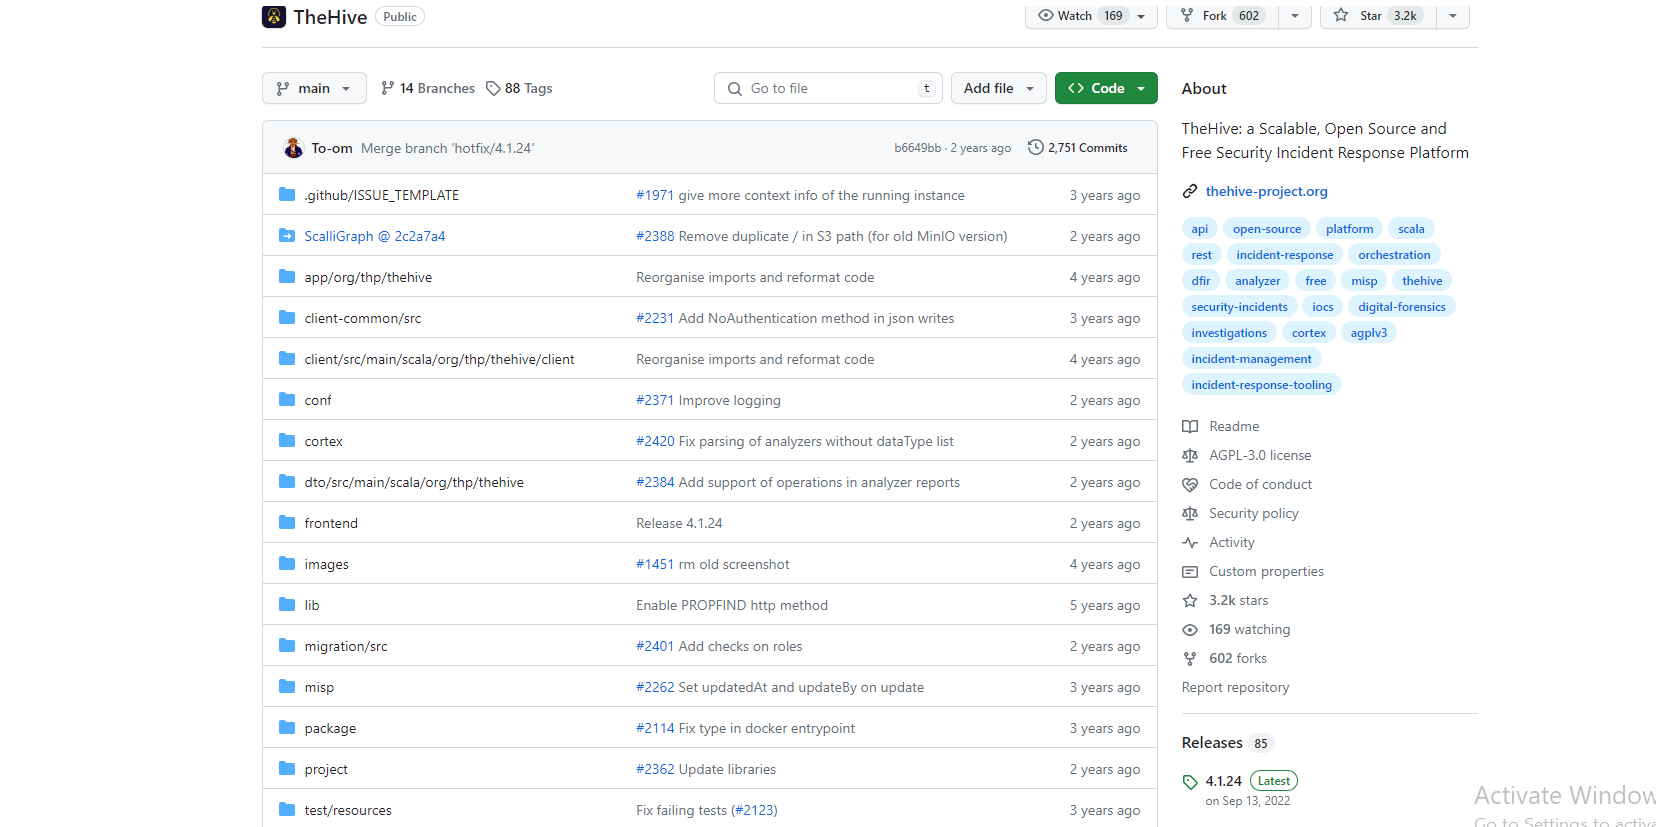
\includegraphics[width=0.8\linewidth]{code.png}
  \caption{The structure of the source code of TheHive}
  \label{fig:source_code_structure}
\end{figure}
We will briefly describe the main modules and packages of the source code in the following subsections.

\subsection{app}

This module contains the core logic and functionality of TheHive. It includes the following packages:

\begin{itemize}
    \item \textbf{org.thp.thehive:} This package contains the main classes and traits that define the application, such as TheHiveApp, TheHiveModule, and TheHiveConfig.
    \item \textbf{org.thp.thehive.controllers:} This package contains the controllers that handle the HTTP requests and responses for the different endpoints of the application, such as Cases, Tasks, Observables, Alerts, and Users.
    \item \textbf{org.thp.thehive.models:} This package contains the case classes and objects that represent the data models of the application, such as Case, Task, Observable, Alert, User, and Organisation.
    \item \textbf{org.thp.thehive.services:} This package contains the services that provide the business logic and operations for the data models, such as CaseSrv, TaskSrv, ObservableSrv, AlertSrv, UserSrv, and OrganisationSrv.
    \item \textbf{org.thp.thehive.connector:} This package contains the classes and traits that enable the integration with external tools and platforms, such as MISP and Cortex.
\end{itemize}

\subsection{client}

This module contains the code for the web-based user interface of TheHive. It includes the following packages:

\begin{itemize}
    \item \textbf{org.thp.thehive.client:} This package contains the classes and objects that define the client-side application, such as ClientApp and ClientConfig.
    \item \textbf{org.thp.thehive.client.pages:} This package contains the components that render the different pages of the user interface, such as DashboardPage, CasePage, TaskPage, ObservablePage, AlertPage, and UserPage.
    \item \textbf{org.thp.thehive.client.services:} This package contains the services that provide the client-side logic and operations for the user interface, such as ApiService, NotificationService, UserService, and OrganisationService.
\end{itemize}
\subsection{conf}

This module contains the configuration files for the application, such as \texttt{application.conf} and \texttt{logback.xml}.

\subsection{cortex}

This module contains the code for the integration with Cortex. It includes the following packages:

\begin{itemize}
    \item \textbf{org.thp.cortex.client:} This package contains the classes and objects that define the client-side communication with Cortex, such as CortexClient and CortexConfig.
    \item \textbf{org.thp.cortex.dto:} This package contains the case classes and objects that represent the data models of Cortex, such as Analyzer, Job, Report, Responder, Action, Response.
\end{itemize}

\subsection{dto}

This module contains the code for the data transfer objects (DTOs) that are used to exchange data between different layers of the application. It includes the following package:

\begin{itemize}
    \item \textbf{org.thp.thehive.dto:} This package contains the case classes and objects that represent the DTOs of TheHive, such as CaseDTO, TaskDTO, ObservableDTO, AlertDTO, UserDTO.
\end{itemize}

\subsection{frontend}

This module contains the code for building and packaging the frontend assets of TheHive. It includes files such as \texttt{webpack.config.js} and \texttt{package.json}.

\subsection{lib}

This module contains some third-party libraries that are used by TheHive. It includes files such as \texttt{scala-graph.jar} and \texttt{elastic4play.jar}.

\subsection{migration}

This module contains some scripts and tools for migrating data from previous versions of TheHive. It includes files such as \texttt{migration.sh} and \texttt{migration.conf}.

\subsection{misp}

This module contains some scripts and tools for synchronizing data with MISP. It includes files such as \texttt{misp.sh} and \texttt{misp.conf}.

\subsection{project}

This module contains some files for managing the project dependencies and build process. It includes files such as \texttt{build.sbt} and \texttt{plugins.sbt}.

\subsection{test}

This module contains some files for testing the application. It includes files such as \texttt{test.conf} and \texttt{test.sh}.

\section{Architecture}
The overall system architecture is composed of the following components:
\begin{figure}[ht]
  \centering
  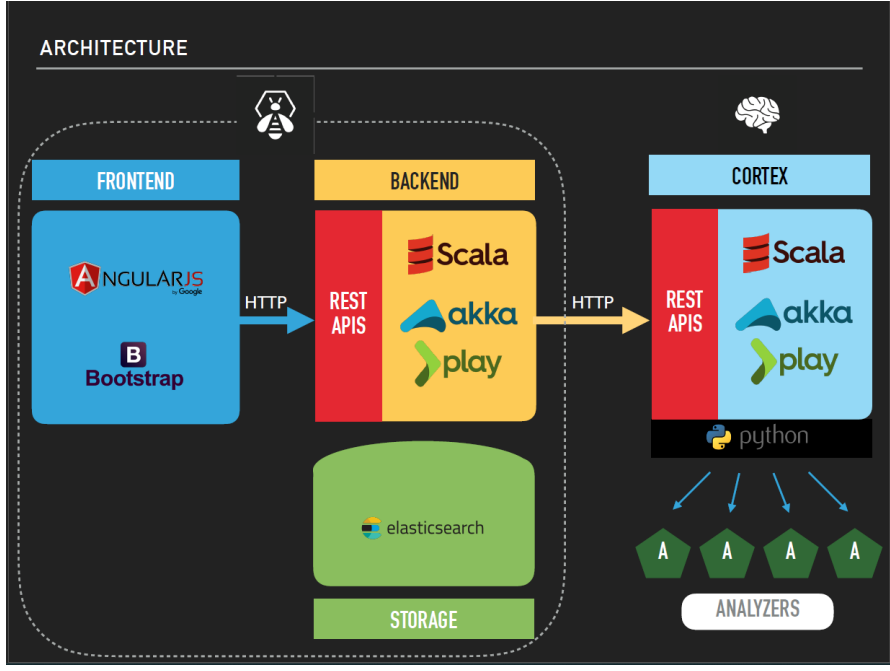
\includegraphics[width=0.8\linewidth]{img1.png}
  \caption{ TheHive Architecture Diagram}
  \label{fig:architecture}
\end{figure}

\begin{itemize}
  \item \textbf{Frontend:} The frontend is responsible for displaying the content of the system to the user. It is built using AngularJS and Bootstrap.

  \item \textbf{Backend:} The backend is responsible for processing the data and providing the data to the frontend. It is built using Scala, Akka, Play Framework, and Slick.

  \item \textbf{Cortex:} Cortex is a real-time streaming analytics platform used to process the data from the backend. It is built using Scala, Akka, Play Framework, and Python.

  \item \textbf{Storage:} The storage layer is employed to store the data from the system. It is comprised of a distributed database, such as Elasticsearch.

  \item \textbf{Analyzers:} The analyzers are utilized to analyze the data from the system. They can perform tasks such as anomaly detection, fraud detection, and trend analysis.
\end{itemize}.



\subsection{Collaboration with Cortex}
TheHive is tightly integrated with Cortex, another powerful tool from TheHive Project. With Cortex, security professionals can conduct in-depth analysis of various types of observables, enhancing incident response efforts through a convenient web interface.

\subsection{Integration with MISP}
TheHive is integrated with MISP (Malware Information Sharing Platform), enhancing its capabilities in handling security incidents.


\subsection{Workflow of TheHive}
\begin{figure}[ht]
    \centering
    \includegraphics[width=0.8\textwidth]{workflow.png}
    \caption{Workflow of TheHive}
    \label{fig:workflow}
\end{figure}

TheHive workflow involves the following key steps:

\begin{enumerate}
    \item \textbf{Create Case Template}: Create a case template to define the structure of incident cases. This includes the fields and attributes that will be used to document and manage incidents.
    \item \textbf{Create Case}: Document and manage incidents by creating cases. Assign cases to analysts or teams for resolution.
    \item \textbf{Create Tasks}: Assign tasks and responsibilities within cases to ensure organized incident response.
    \item \textbf{Create Alerts}: Create alerts to notify analysts of potential security incidents.
    \item \textbf{Create Observables}: Create observables to document and analyze potential threats associated with incidents.
    \item \textbf{Run Analyzers}: Use various analyzers to gather additional information and context about incidents and associated observables.
    \item \textbf{Create Logs}: Create logs to document actions taken by analysts during incident response.
    \item \textbf{Create Analysis Reports}: Use analysis reports to document findings and conclusions about incidents and observables.
    \item \textbf{Create Jobs}: Create jobs to automate incident response tasks.
    \item \textbf{Create Report Templates}: Create report templates to document incident response activities and outcomes.
\end{enumerate}




\section{Documentation to run Features}
TheHive has many amazing functionalities that make it a powerful tool for security incident response. Here we will discuss some of the most important ones.


\subsection{Admin side}
TheHive is a web application that can be installed on a server and accessed from a web browser. It has a web-based administration interface that allows administrators to configure the tool according to their needs. Administrators can create users, assign roles to them, and manage their permissions. They can also configure the tool to send notifications via email or SMS when certain events occur, such as new incidents being created or updated, or when certain actions are performed by users, such as adding comments or attachments to incidents.
list of features:
\begin{itemize}
\item Organization management
\item Link organizations
\item Account management
\item Entities 
\item Permission management
\item Observables types
\item Case Status
\item Alert Status
\end{itemize}

\subsubsection*{Organization management}
\subsubsection{Create an Organization}

TheHive allows administrators to create multiple organizations within the tool. Each organization can have its own set of users, roles, permissions, and notifications. This allows for better separation of duties and responsibilities between different teams within an organization, such as a SOC team and a CSIRT team.\\

\begin{figure}[ht]
    \centering
    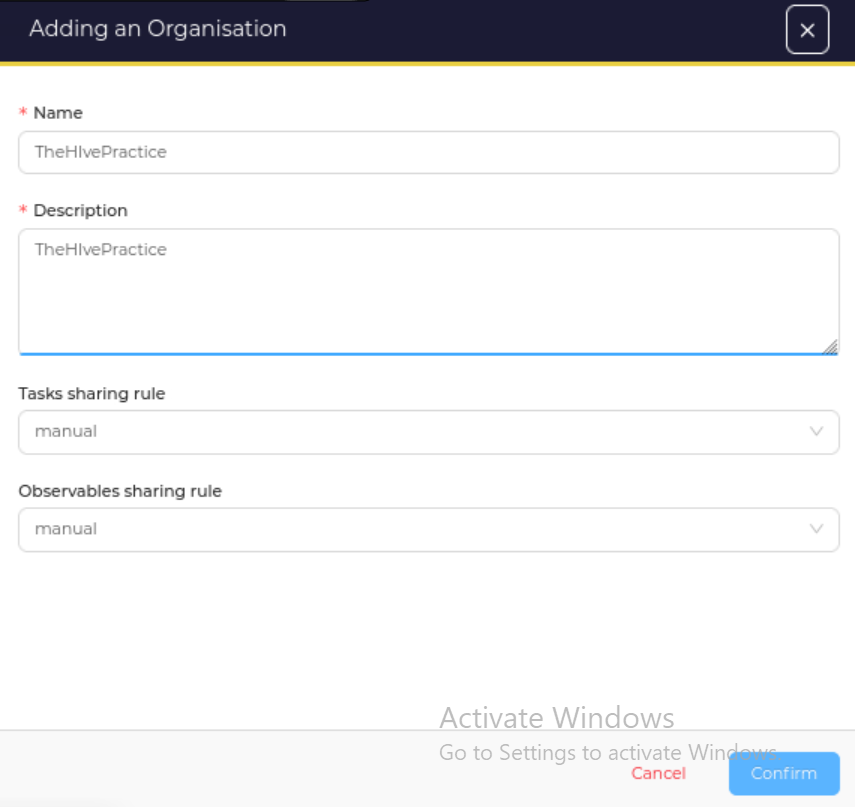
\includegraphics[width=0.8\textwidth]{img14.png}
    \caption{Create An Organization}
    \label{fig:org}
\end{figure}\\
\begin{figure}[ht]
    \centering
    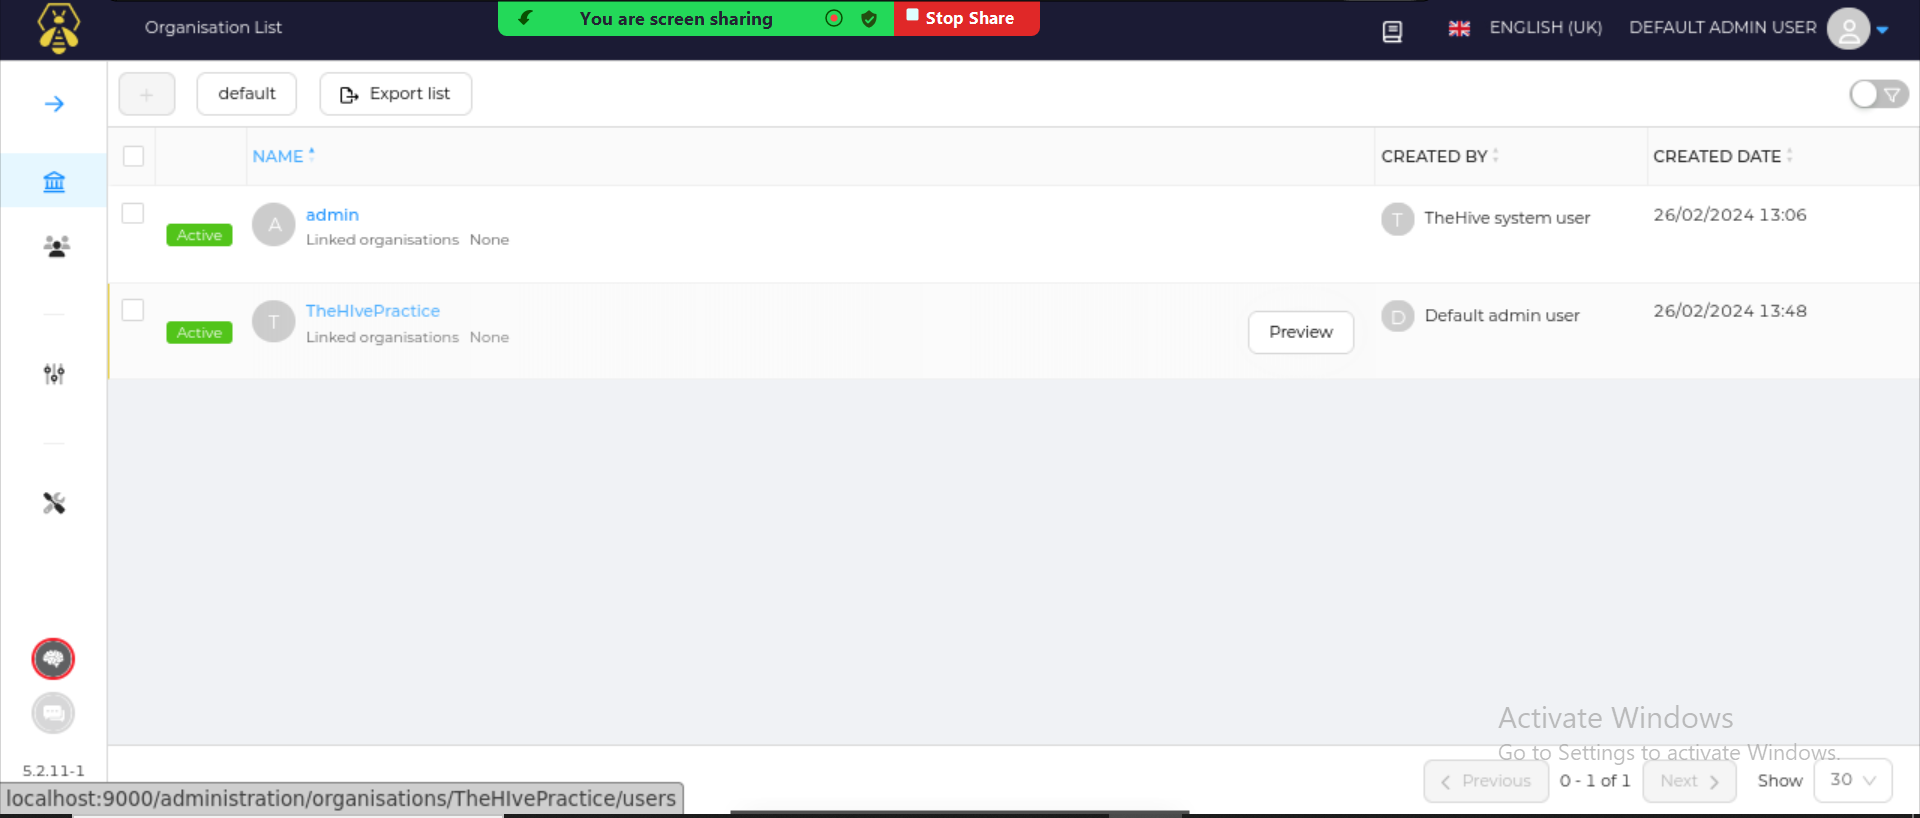
\includegraphics[width=0.8\textwidth]{img15.png}
    \caption{Organization Management}
    \label{fig:org}
\end{figure}\\
To create a new organization, follow these steps: \\
1. Click on the \textbf{Add an Organization} button.\\
2. Edit the required fields in the drawer:
    \begin{itemize}
        \item A placeholder exists and a logo of the Organisation can be added.
        \item Name: Name of the new Organization.
        \item Description: Description for the new Organization.
        \item Task sharing rule: default sharing rule for Tasks that will be applied when a Case will be shared with another Organization.
        \item Observables sharing rule: default sharing rule for Observables that will be applied when a Case will be shared with another Organization.
    \end{itemize}
3. Click \textbf{Confirm} to create the organization.

We can see this in Figure \ref{fig:org} that organization is created.


\subsubsection{Link Organization}

TheHive allows administrators to link multiple organizations together. This allows for better collaboration between different teams within an organization, such as a SOC team and a CSIRT team.\\
To link an organization, follow these steps: \\

Here are the steps to manage links in TheHive:

1. Open the detailed view of an Organization.\\
2. Open the Linked Organization tab.\\

We can see this in Figure \ref{fig:link}.

\begin{figure}[ht]
    \centering
    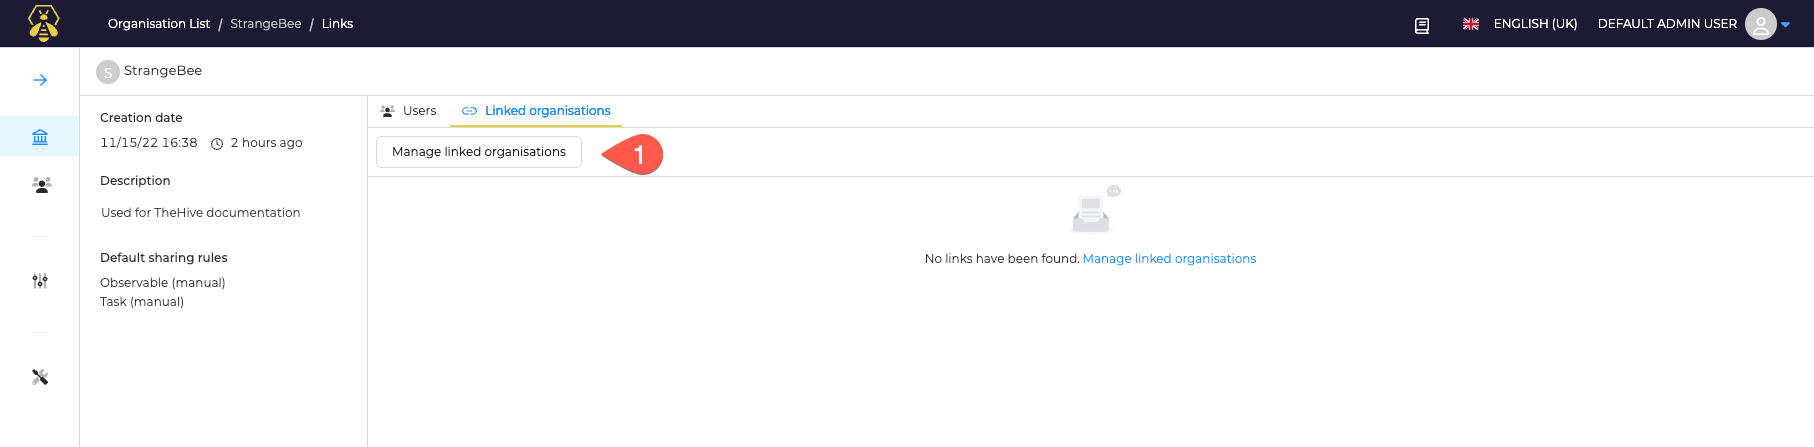
\includegraphics[width=0.8\textwidth]{img17.png}
    \caption{Link Organization}
    \label{fig:link}
\end{figure}

3. Click on the button named \textbf{Manage linked Organizations}.\\

We can see this in Figure \ref{fig:manage}.\\
\begin{figure}[h!]
    \centering
    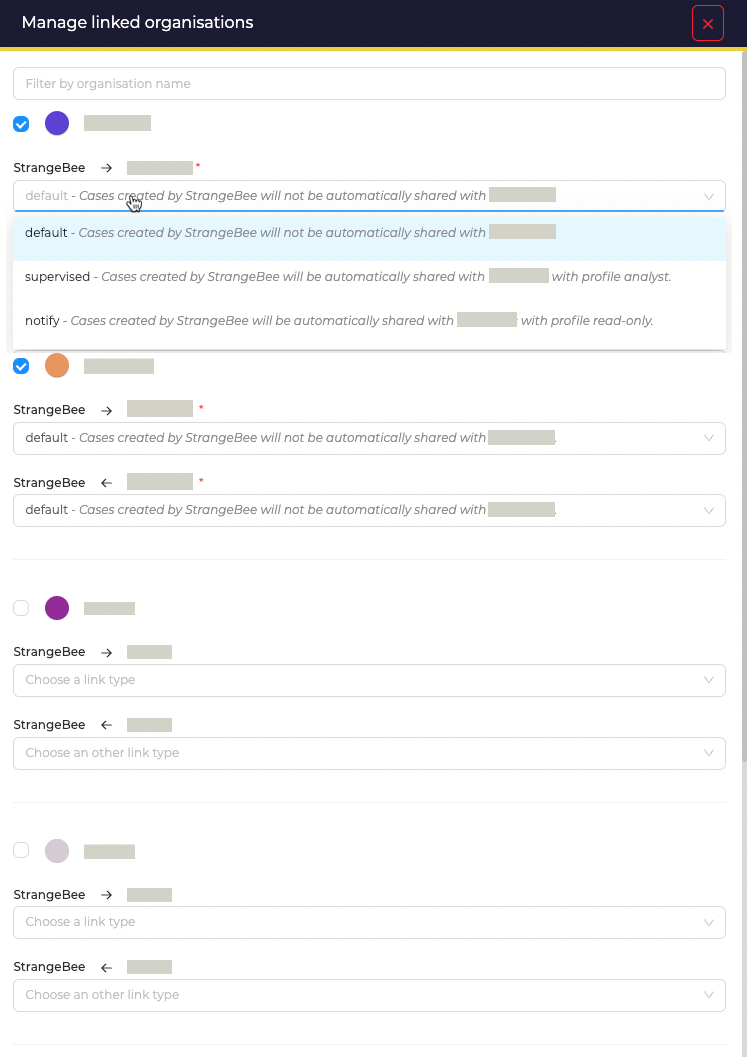
\includegraphics[width=0.8\textwidth]{img16.png}
    \caption{Manage Link Organization}
    \label{fig:manage}
\end{figure}
4. For each other organization, select:\\
    \begin{itemize}
        \item If you want the current Organization to be linked with it.
        \item The types of link that should be created.
    \end{itemize}
3 types of links are available:

\begin{itemize}
    \item default: Cases created by the current Organisation will not be shared with the other one.
    \item supervised: Cases created by the current Organisation will be automatically shared with the other one, with the profile Analyst.
    \item notify: Cases created by the current Organisation will be automatically shared with the other one, with the profile Read-only.
\end{itemize}

\subsection{Account Management}
TheHive allows administrators to create multiple user accounts within the tool. Each user account can have its own set of roles and permissions. This allows for better separation of duties and responsibilities between different users within an organization, such as a SOC team and a CSIRT team.\\
Accounts can be created or edited from several places in TheHive:

\begin{enumerate}
  \item As Administrator, in the Users view
  \item As Administrator in the detailed page of an Organisation
  \item As Org-admin, in the Organisation configuration page

\end{enumerate}
 \\
We can see this in Figure \ref{fig:users}.
\begin{figure}[h!]
    \centering
    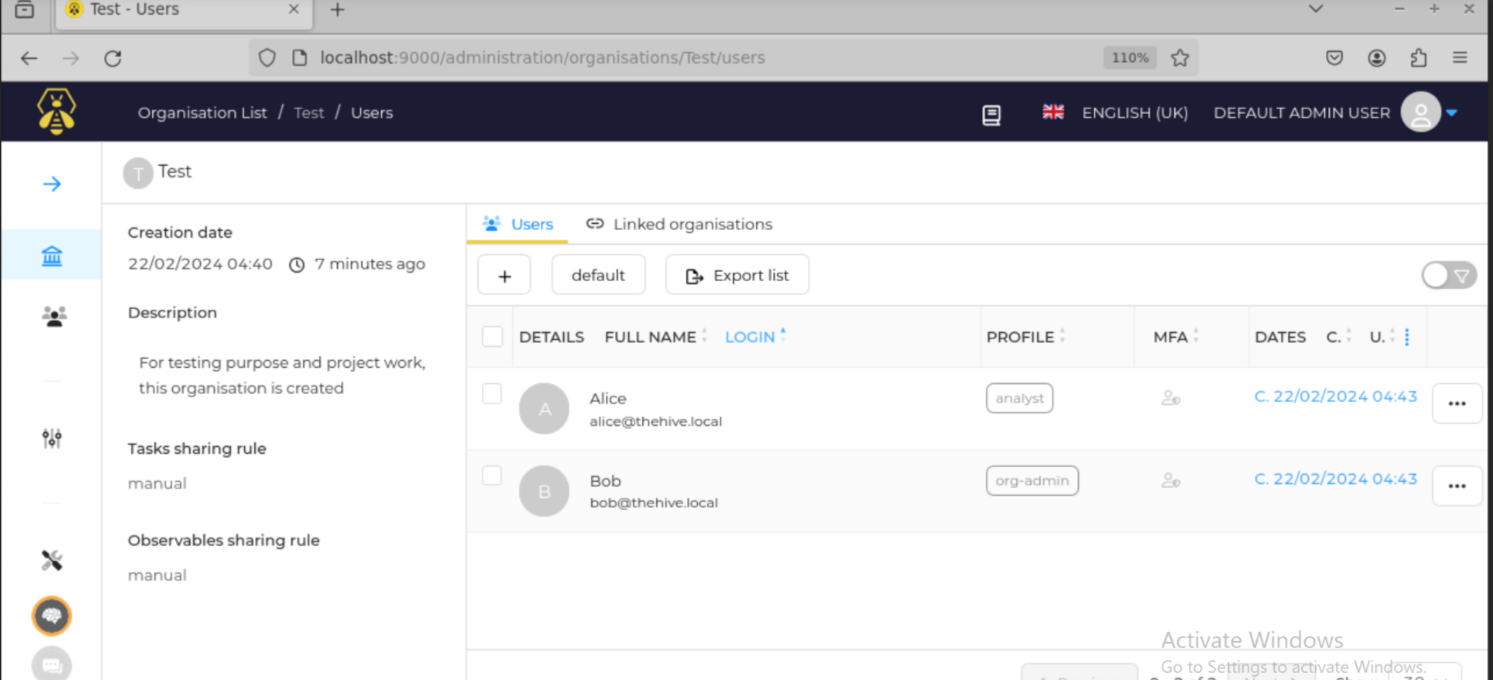
\includegraphics[width=0.8\textwidth]{img3.png}
    \caption{Users}
    \label{fig:users}
\end{figure}

Starting with TheHive 5.0, two types of accounts exist in the application:

\begin{enumerate}
  \item Normal accounts: These are used for standard users, such as analysts. These accounts can be used to open a session on the web UI, utilize all available authentication methods, and API keys if enabled.
  
  \item Service accounts: These are recommended for use by accounts in charge of automation within the application, such as those used to create Alerts. Service accounts can only be used to authenticate the application through the API, using an API key.
\end{enumerate}

Click on the \textbf{Add a User} button. \\
To create an account:\\
\begin{figure}[h!]
    \centering
    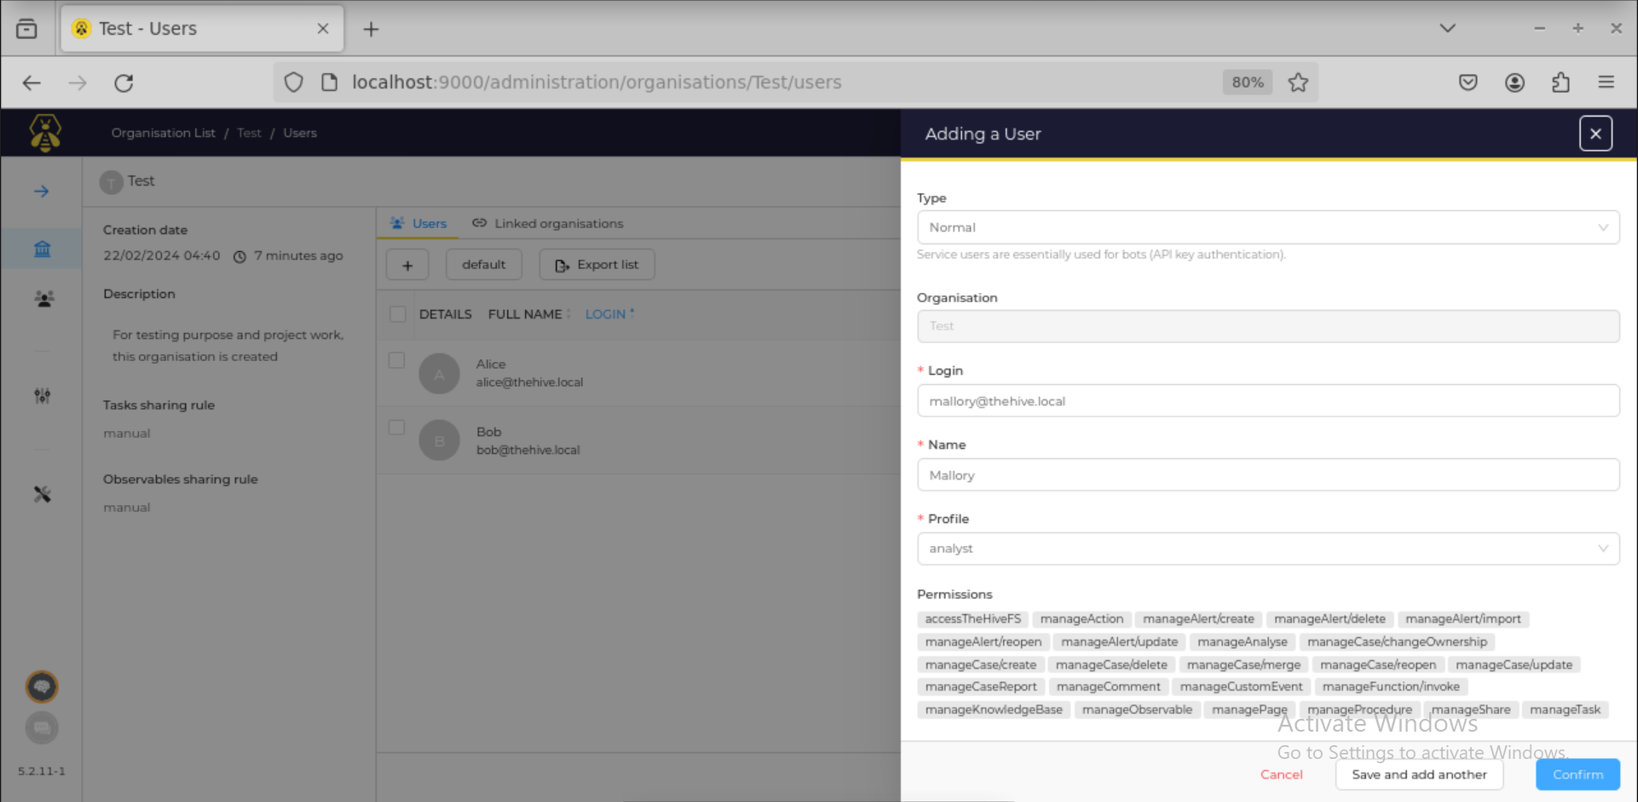
\includegraphics[width=0.8\textwidth]{img4.png}
    \caption{Add User}
    \label{fig:add}
\end{figure}



\begin{enumerate}
  \item Choose the type of account, either Normal or Service.
  \item Fill in the login name (formatted as an email address).
  \item Specify a name for the account.
  \item Select the organizations and associated profiles for this account.
  \item Click on "Set as default" to define the default organization for the account.
  \item Finally, click "Confirm."
\end{enumerate}
\begin{figure}[h!]
    \centering
    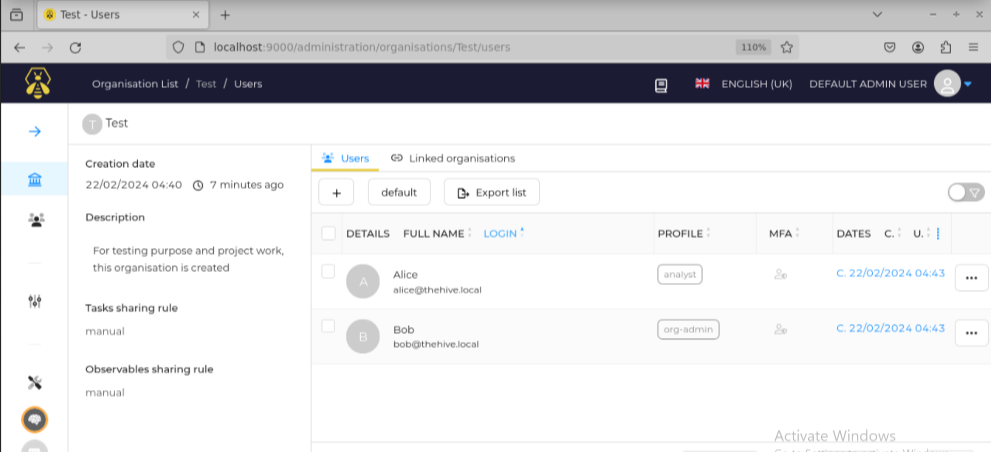
\includegraphics[width=0.8\textwidth]{img5.png}
    \caption{Successful Creation of User}
    \label{fig:add}
\end{figure}

We can see The final look after creating Users in Figure \ref{fig:add}.
We can also edit an existing account by clicking on the \textbf{preview} button. \\

\subsection{Entities \& Permissions}
TheHive comes with a set of predefined profiles for Administrators and Organsations ; this set can be enriched with custom profiles you can create depending on your needs.\\
We can see this in Figure \ref{fig:entities}.
\begin{figure}[h!]
    \centering
    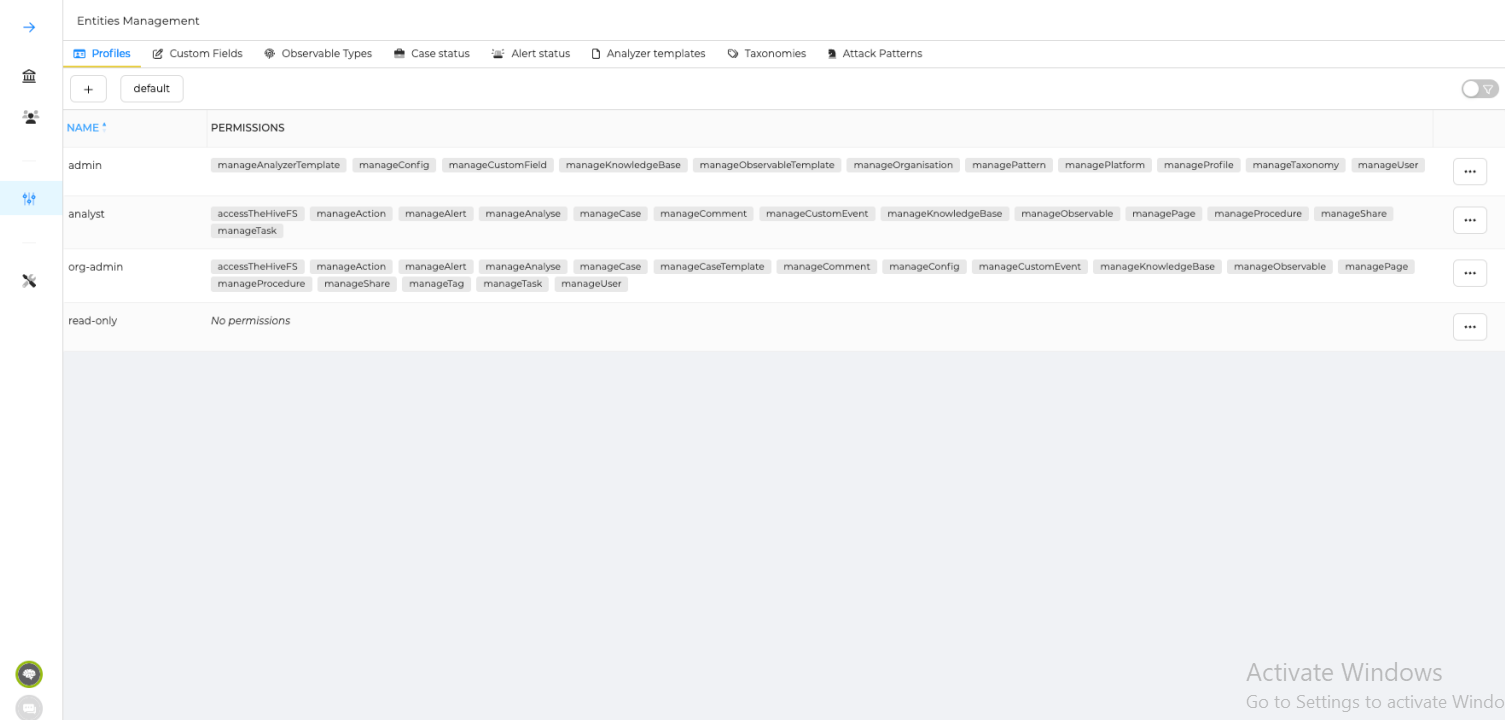
\includegraphics[width=0.8\textwidth]{img6.png}
    \caption{Entities avaliable}
    \label{fig:entities}
\end{figure}

Users are given Permissions by their roles. \\
Permissions are defined for each entity of the application.\\
The following entities are available:
\begin{itemize}
    \item admin
    \item analyst
    \item org-admin
    \item read-only
\end{itemize}

\subsection{Users Roles}
Now that we have created our users, we need to assign them roles.\\
We have the entities given in Figure \ref{fig:entities}. We can give roles according to our needs.\\
\begin{enumerate}
    \item \textbf{Admin}:
       \begin{itemize}
         \item \textbf{Description}: Administrators have full control over TheHive platform. They can create, modify, and delete accounts, organizations, and configurations. Administrators typically manage the overall settings and ensure the platform functions smoothly.
         \item \textbf{Privileges}:
         \begin{itemize}
           \item Full access to all features and functionalities.
           \item User and organization management.
           \item Configuration and system settings control.
           \item Incident case management.
         \end{itemize}
       \end{itemize}
  
    \item \textbf{Analyst}:
       \begin{itemize}
         \item \textbf{Description}: Analysts are standard users responsible for working on incident cases and investigations within TheHive. They have access to case management and analysis tools to investigate and respond to security incidents.
         \item \textbf{Privileges}:
         \begin{itemize}
           \item Access to incident case management.
           \item Ability to work on and update cases.
           \item Collaboration with other analysts.
           \item Limited access to system configurations.
         \end{itemize}
       \end{itemize}
  
    \item \textbf{Org-admin} (Organization Administrator):
       \begin{itemize}
         \item \textbf{Description}: Organization administrators have administrative privileges limited to a specific organization within TheHive. They can manage users, incidents, and configurations for their assigned organization.
         \item \textbf{Privileges}:
         \begin{itemize}
           \item User management within their organization.
           \item Incident case management within their organization.
           \item Limited access to system-wide configurations.
           \item May not have access to other organizations' data.
         \end{itemize}
       \end{itemize}
  
    \item \textbf{Read-only}:
       \begin{itemize}
         \item \textbf{Description}: Read-only users have limited access and are primarily meant for users who need to view incident cases and data without making changes or updates. They can review and gather information but cannot modify cases.
         \item \textbf{Privileges}:
         \begin{itemize}
           \item View-only access to incident cases and data.
           \item Cannot modify or update cases.
           \item Limited interaction with the platform.
         \end{itemize}
       \end{itemize}
  \end{enumerate}
  \subsection{Cases}
A case furnishes details about potentially suspicious activity within an environment. It encompasses information regarding security incidents, observables, alerts, and impacted users. Security analysts utilize cases for targeted analyses, evaluating the potential threats present. Cases can originate from diverse sources and typically include a title, tags, task rules, observable rules, a detailed description of case specifics, and all pertinent details essential for constructing a rationale to identify and address specific threats.\\
After logging into an user account ,a user can see the list of cases of his
organization. It is shown in figure\\
\begin{figure}[ht]
    \centering
    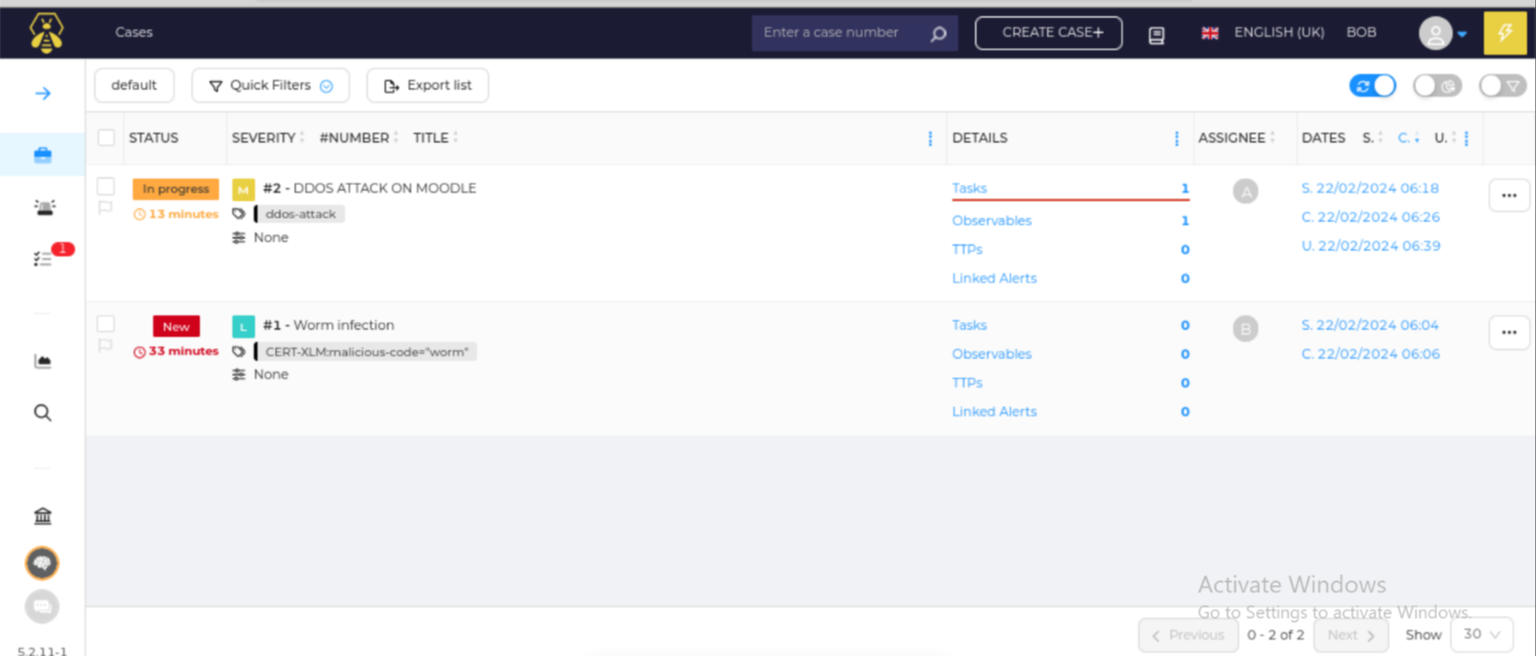
\includegraphics[width=0.8\textwidth]{img7.png}
    \caption{Cases}
    \label{fig:entities}
\end{figure}

\subsubsection*{Create a Case}

To create new cases using templates, follow these steps:

\begin{enumerate}
  \item Click on "Create Case +" located in the header.

\begin{figure}[H]
    \centering
    
\includegraphics[width=0.8\textwidth]{img18.png}
    \caption{Create Case}
    \label{fig:createcase}
\end{figure}

  \item Cases can be created from the following. Either of these can be selected.
\begin{itemize}
    \item Empty Case
    \item Case Template
    \item Archive
    \item From MISP (.json)

\end{itemize}

It can be shown in Figure \ref{fig:casefrom}.
\begin{figure}[H]
    \centering
    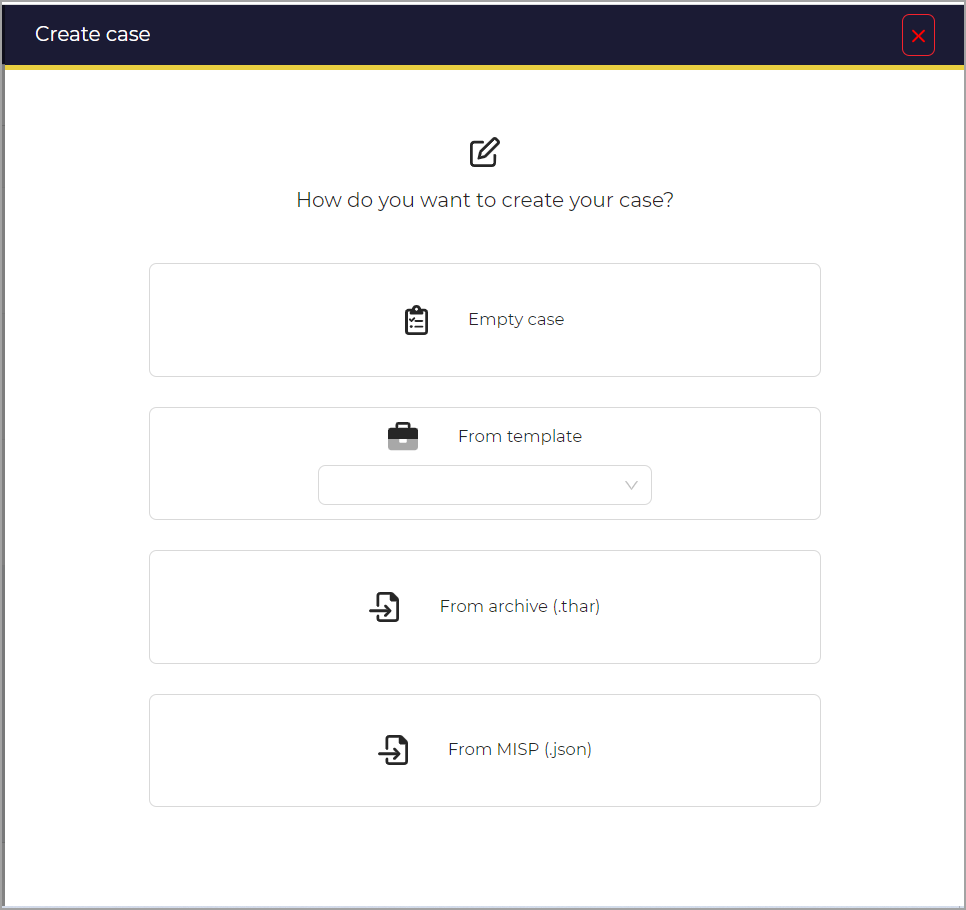
\includegraphics[width=0.8\textwidth]{img19.png}
    \caption{Create Case from}
    \label{fig:casefrom}
\end{figure}

\end{enumerate}
We will create case from empty case.\\

\subsubsection*{Creating a New Case from an Empty Case}

To create a new case from an empty case, these steps are followed:

\begin{itemize}
  \item Enter the case title in the "Title" field.
  \item Select a date from the "Date" field.
  \item Select the severity level (Low/Medium/High/Critical).
  \item Select the TLP (Traffic Light Protocol) level (White/Green/Amber/Red).
  \item Select the PAP (Perceived Attribution Program) level (White/Green/Amber/Red).
  \item Click the "+" button to add tags (refer to "Add Tags").
  \item Enter the case description in the "Description" field.
  \item Choose a Task rule from the list (manual/existingOnly/upcomingOnly/all).
  \item Choose an Observable rule from the list (manual/existingOnly/upcomingOnly/all).
  \item Add tasks (refer to "Add Tasks").
  \item Add custom fields (refer to "Add Custom Field Values").
  \item Click the "Confirm case creation" button to create the case.
\end{itemize}

It can be shown in Figure \ref{fig:emptycase}.
\begin{figure}[H]
    \centering
    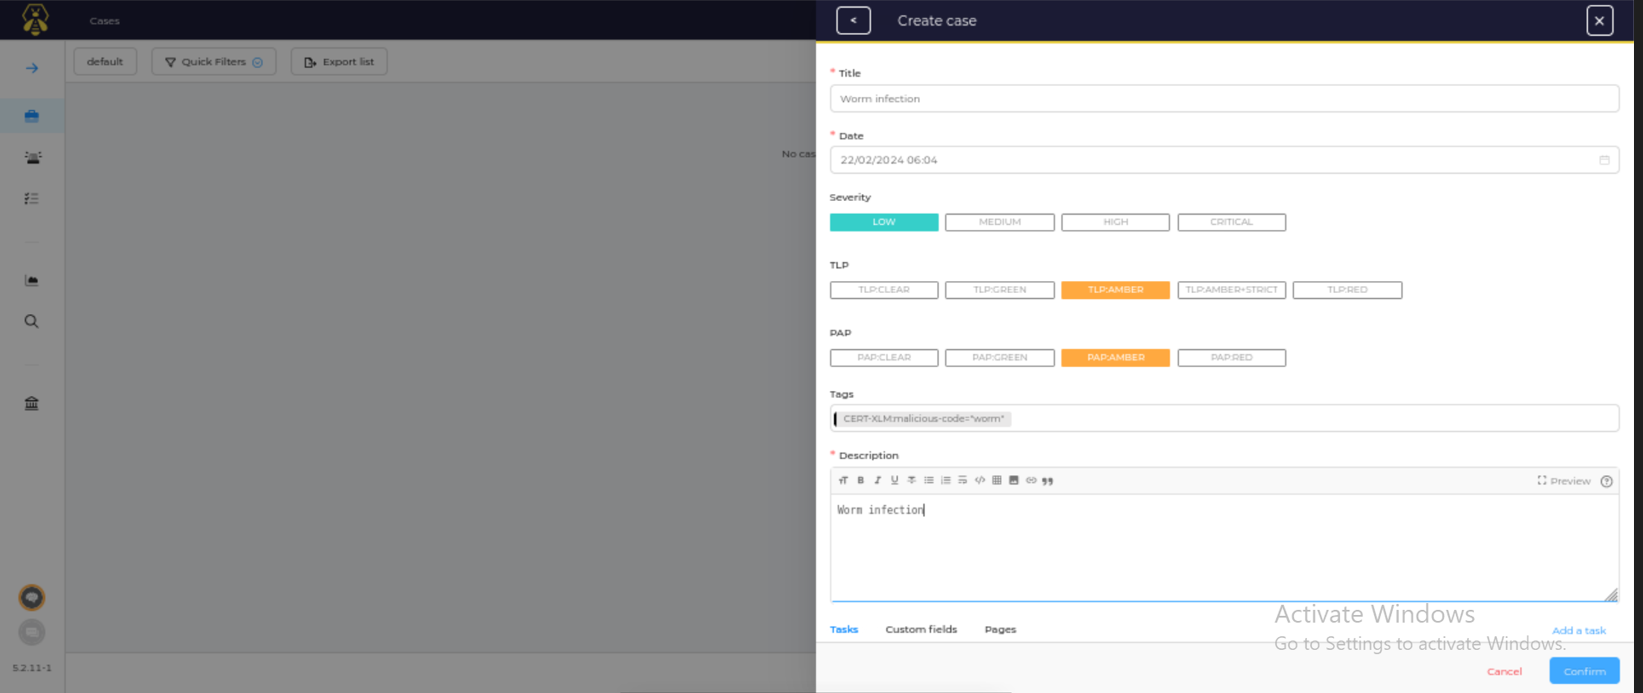
\includegraphics[width=0.8\textwidth]{img9.png}
    \caption{Empty Case}
    \label{fig:emptycase}
\end{figure}
\subsubsection*{Statistics}
We can view the statistics by enabling the stats toggle button
\begin{figure}[H]
    \centering
    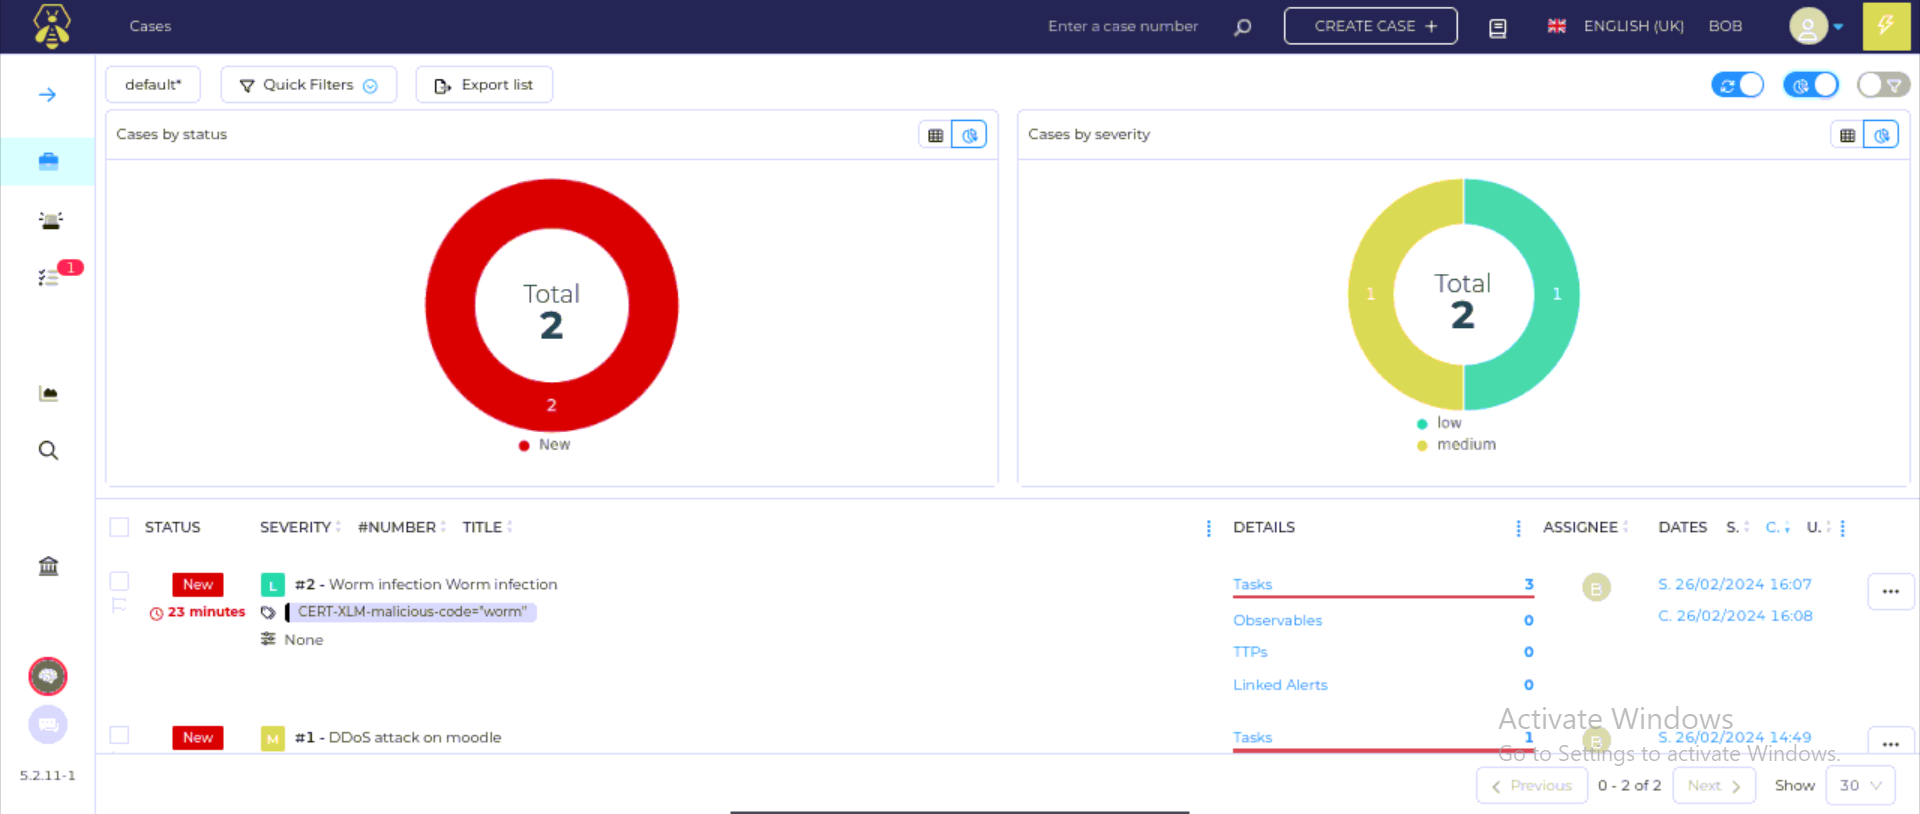
\includegraphics[width=0.8\textwidth]{img32.png}
    \caption{Statistics}
    \label{fig:emptycase}
\end{figure}

\subsection{Task}
After creating a new case ,a user can create tasks which should be performed
to resolve the case and assign those tasks to different users. So,For a
particular case while adding a task we need to fill up the following dialogbox
with necessary information about that task
\begin{figure}[H]
    \centering
    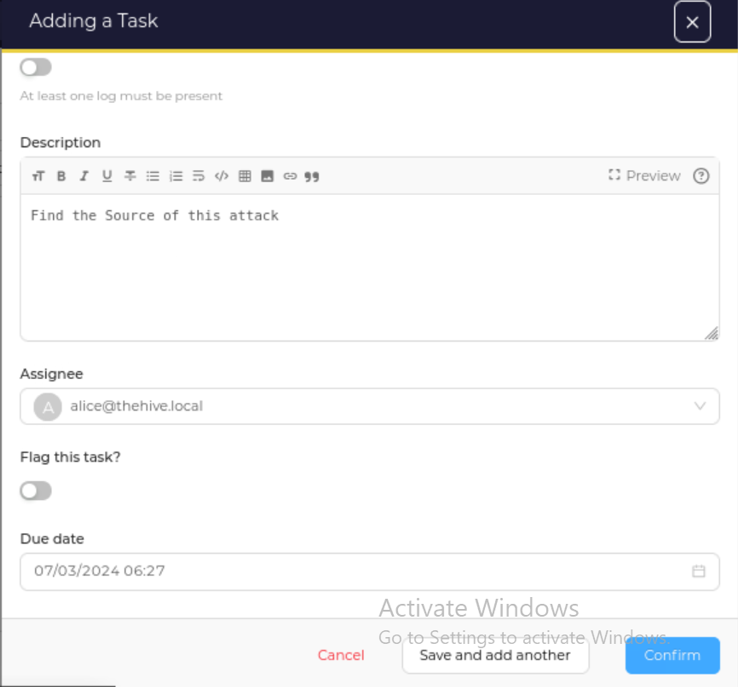
\includegraphics[width=0.8\textwidth]{img12.png}
    \caption{Adding a task}
    \label{fig:entities}
\end{figure}
Then after creating a task successfully the dashboard of a case under
”Tasks” tab will look like below
\begin{figure}[H]
    \centering
    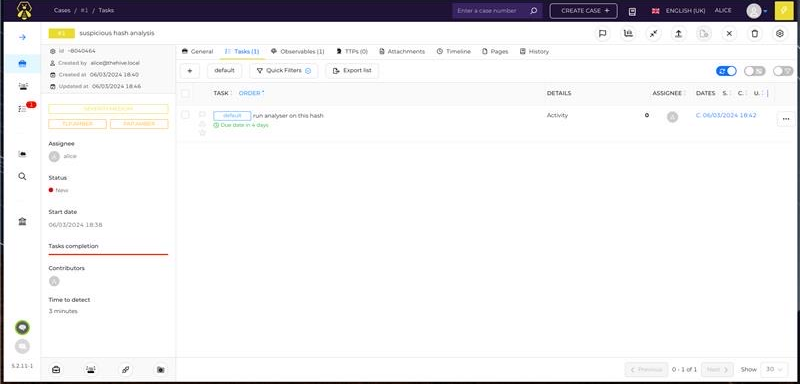
\includegraphics[width=0.8\textwidth]{img38.png}
    \caption{Case dashboard(after adding a new task)}
    \label{fig:entities}
\end{figure}



  \subsection{Observables types}
Administrators using The Hive have the flexibility to establish various observable types, each equipped with its unique attributes. This feature enables a more efficient distribution of tasks and responsibilities among distinct teams within an organization, fostering improved collaboration between, for instance, a Security Operations Center (SOC) team and a Computer Security Incident Response Team (CSIRT).\\
The following steps creates a new observable type: \\
\begin{enumerate}
\item  Click on the \textbf{Add an Observable Type} button.
\item  Edit the required fields in the drawer:
   \begin{itemize}
        \item Name: Name of the new Observable Type.
        \item Description: Description for the new Observable Type.
        \item Attribute: Attribute for the new Observable Type.
    \end{itemize}
\item Click \textbf{Confirm} to create the observable type.
\end{enumerate}

We can see this in Figure \ref{fig:observables}.
\begin{figure}[H]
    \centering
    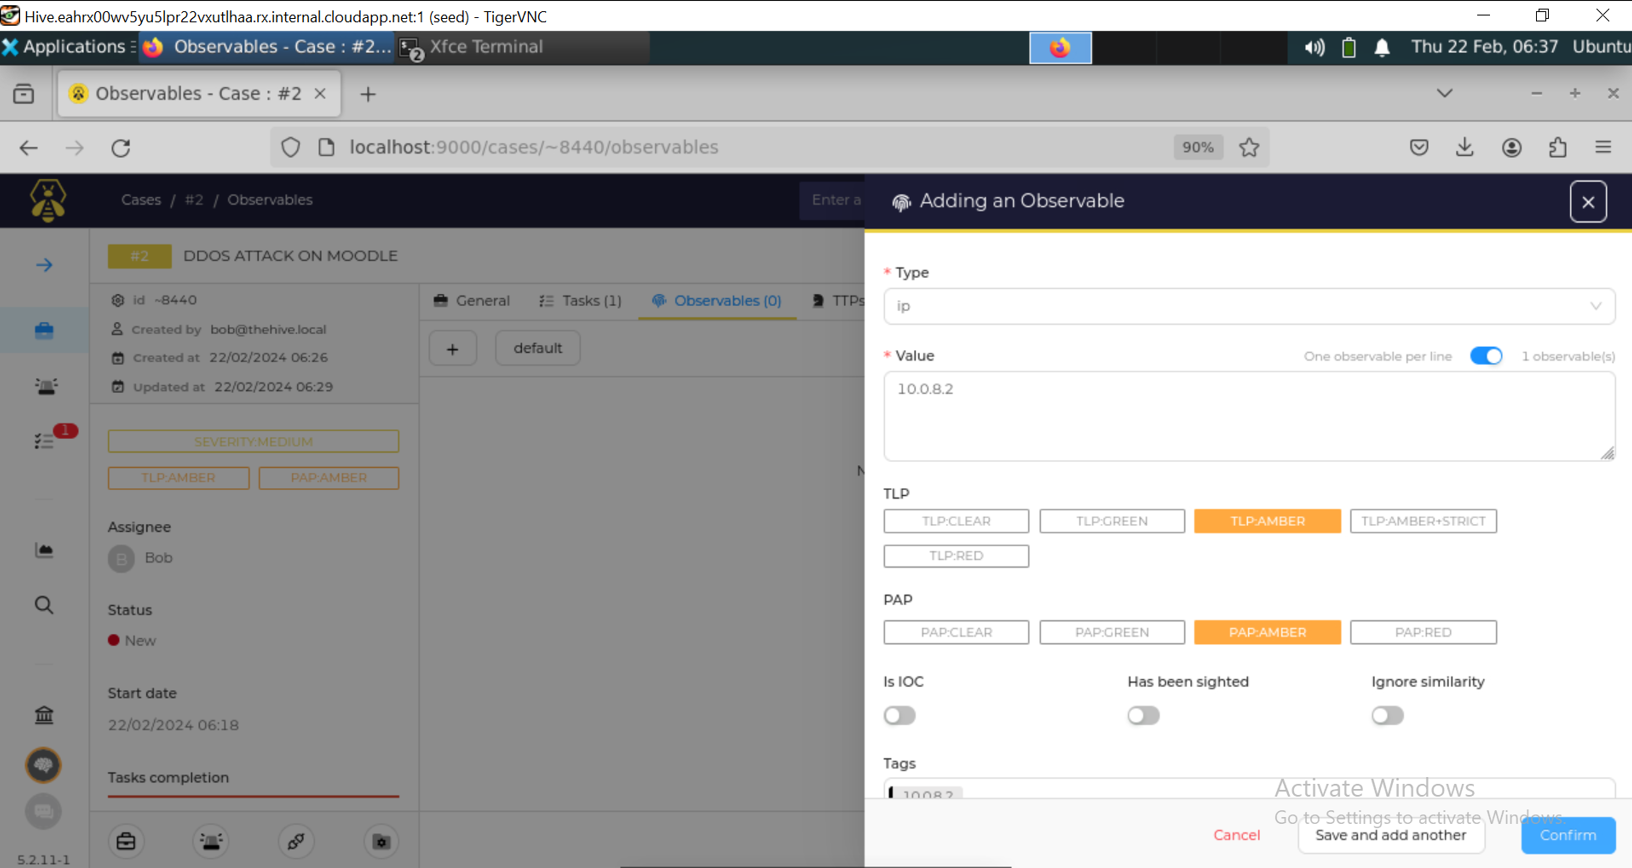
\includegraphics[width=0.8\textwidth]{img20.png}
    \caption{Create Observables}
    \label{fig:observables}
\end{figure}

After creating observables we cam find the list of observables for a particular case. It is shown in \ref{fig:observablesList}

\begin{figure}[H]
    \centering
    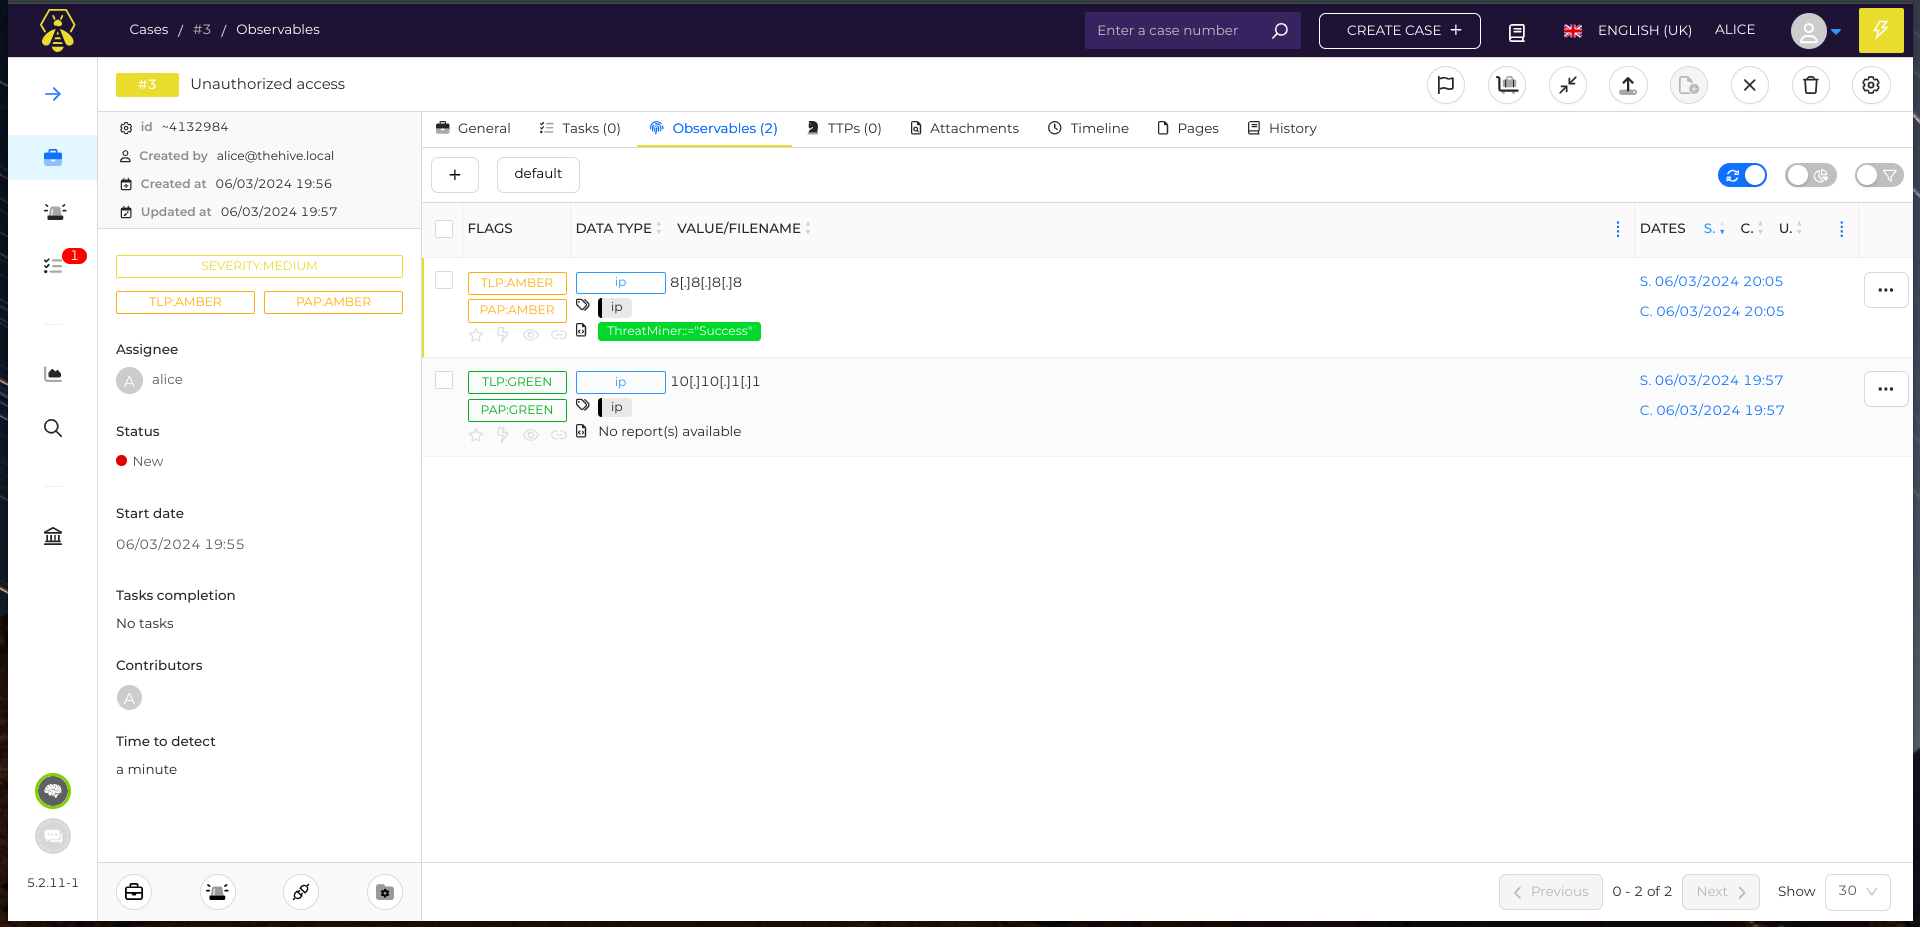
\includegraphics[width=0.8\textwidth]{img37.png}
    \caption{Observables list}
    \label{fig:observablesList}
\end{figure}


\subsection{Cases and Alert Status}
Admin also have the capability to introduce new statuses for both cases and alerts. Admin must provide the following details to define a status:

\begin{enumerate}
  \item \textbf{Stage}: select the stage of the new status.
  \item \textbf{Value}: select a name for the new status.
  \item \textbf{Color}: select a color for users to quickly identify the status 
\end{enumerate}

for example:

\begin{itemize}
  \item \textbf{Stage}: Investigation
  \item \textbf{Value}: In Progress
  \item \textbf{Color}: \textcolor{red}{Red}
\end{itemize}

Here, for the "Investigation" stage a status "Processing" is defined with a red color for users to quickly identify the status.


\subsection{User side}
TheHive boasts a user-friendly web interface facilitating tool access from any Internet-connected computer. Users can initiate incidents, augment them with comments and attachments, delegate tasks to peers, and conclude incidents upon resolution. Additionally, users have the capability to conduct targeted searches for incidents based on criteria like status, severity level, or creation date. The tool offers diverse features, including:
list of features:
\begin{itemize}
\item Incident management
\item Case management
\item Task management
\item Report management
\item Dashboard management
\item Integration with other tools
\end{itemize}

\subsubsection{Templetes}
As an organization administrator, you have the ability to craft templates for various components such as incidents, cases, pages, and reports. Following is the process of creating templates specifically for cases:
First, let's see the lists of case templetes.\\

\begin{itemize}
\item Access to the list by opening the Organisation menu, then the Templates tab, and the Cases tab. It is shown in Figure \ref{fig:templetes} 

\begin{figure}[h!]
    \centering
    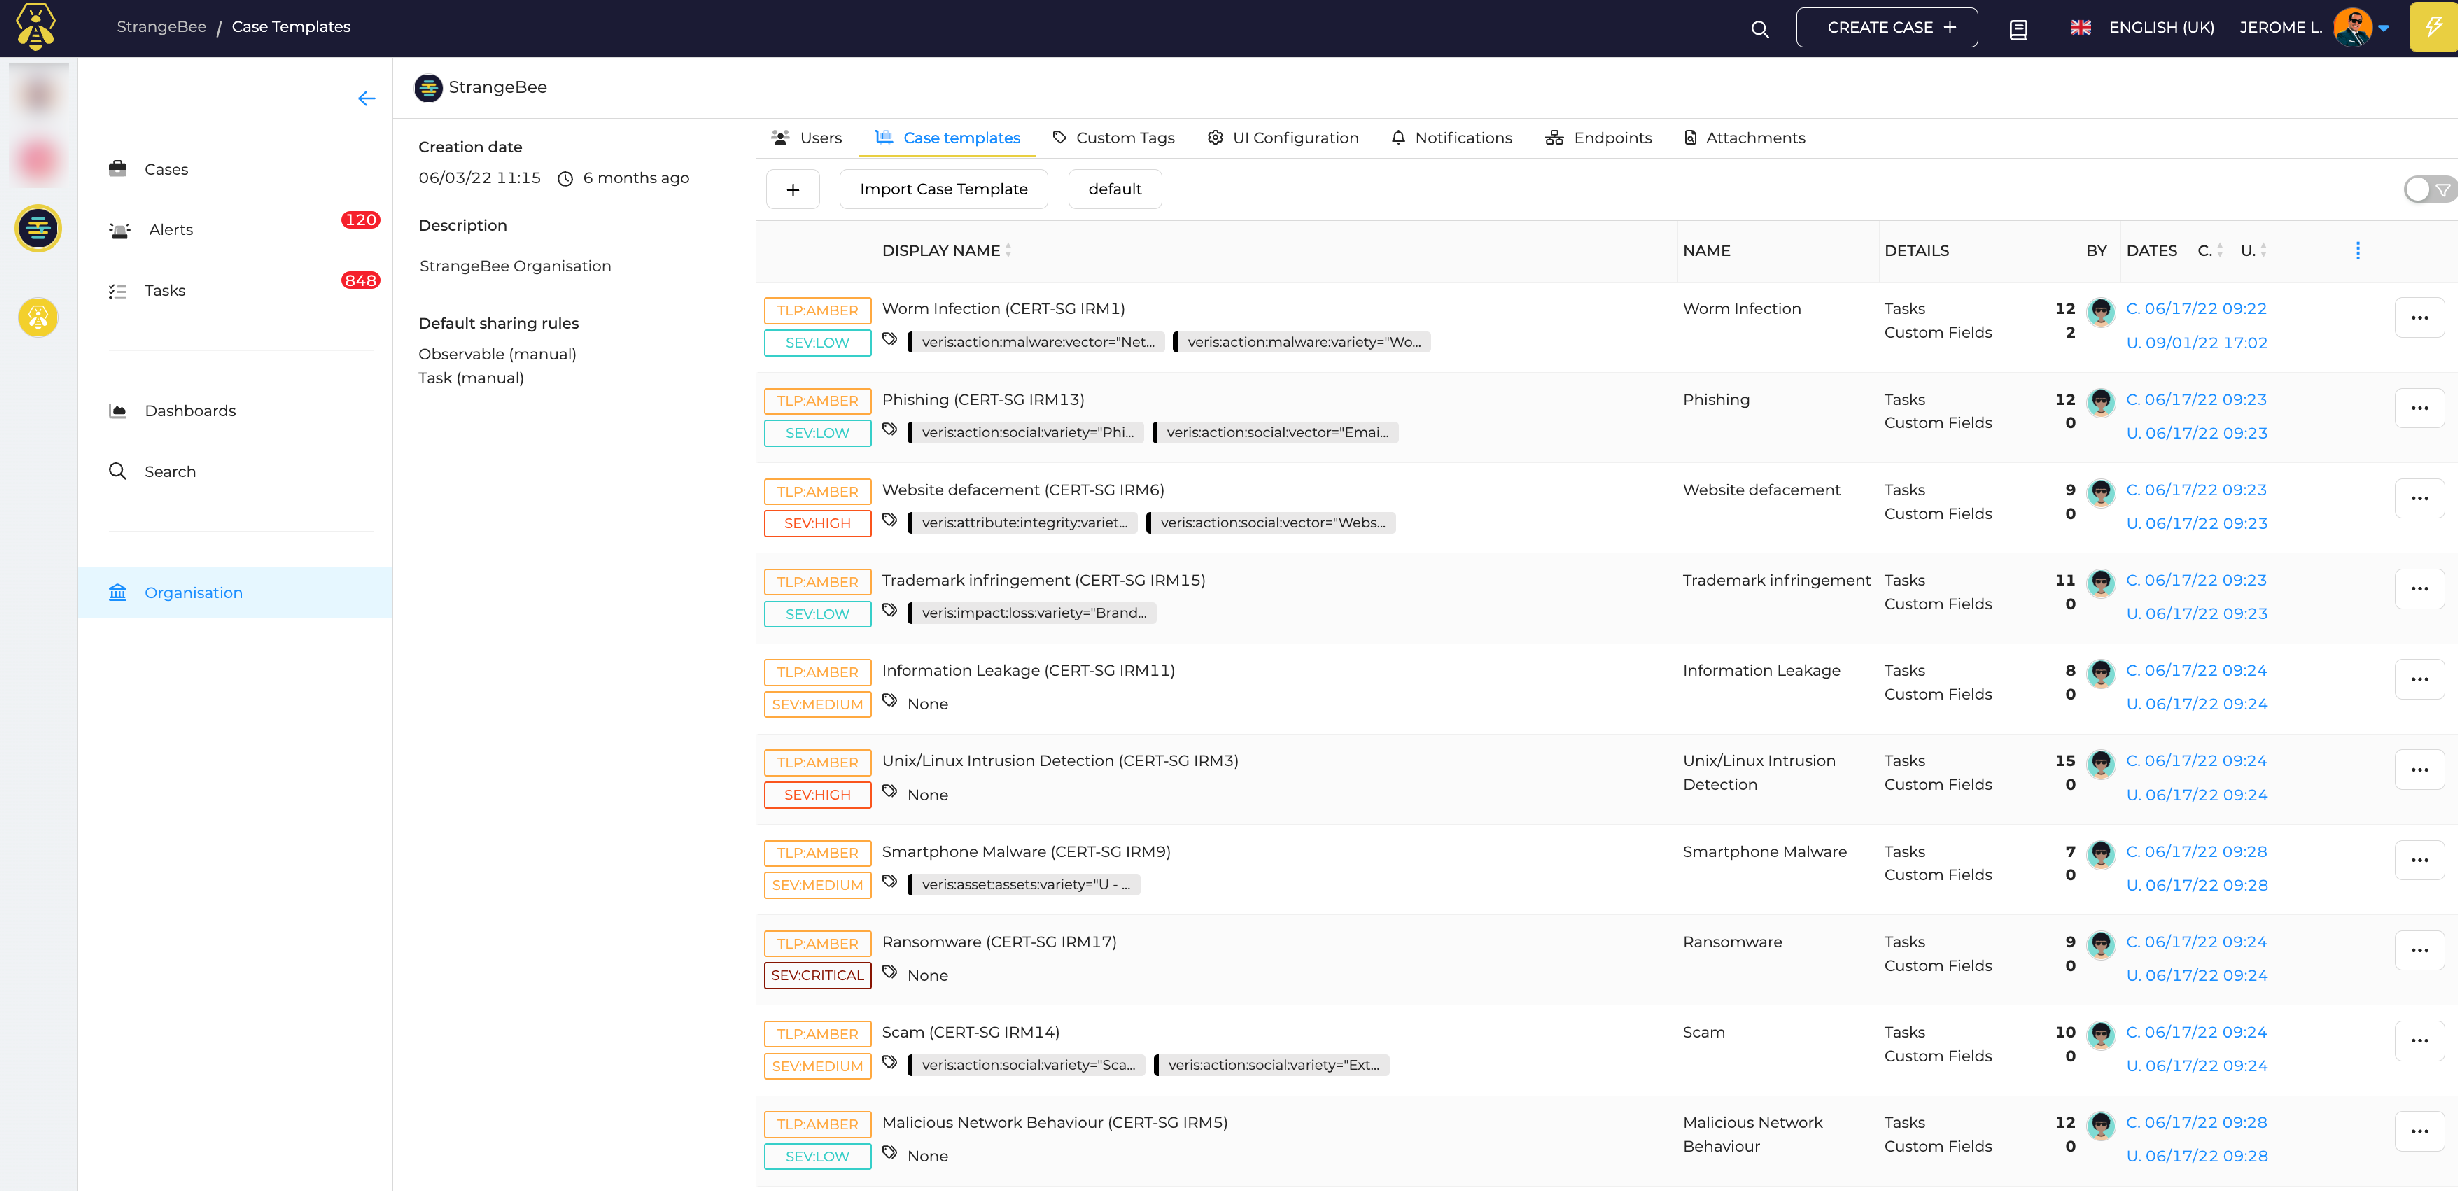
\includegraphics[width=0.8\textwidth]{img21.png}
    \caption{List of Case templates}
    \label{fig:templetes}
\end{figure}

\item Click the plus button to create a new Case template. It is shown in Figure \ref{fig:new}.
\begin{figure}[h!]
    \centering
    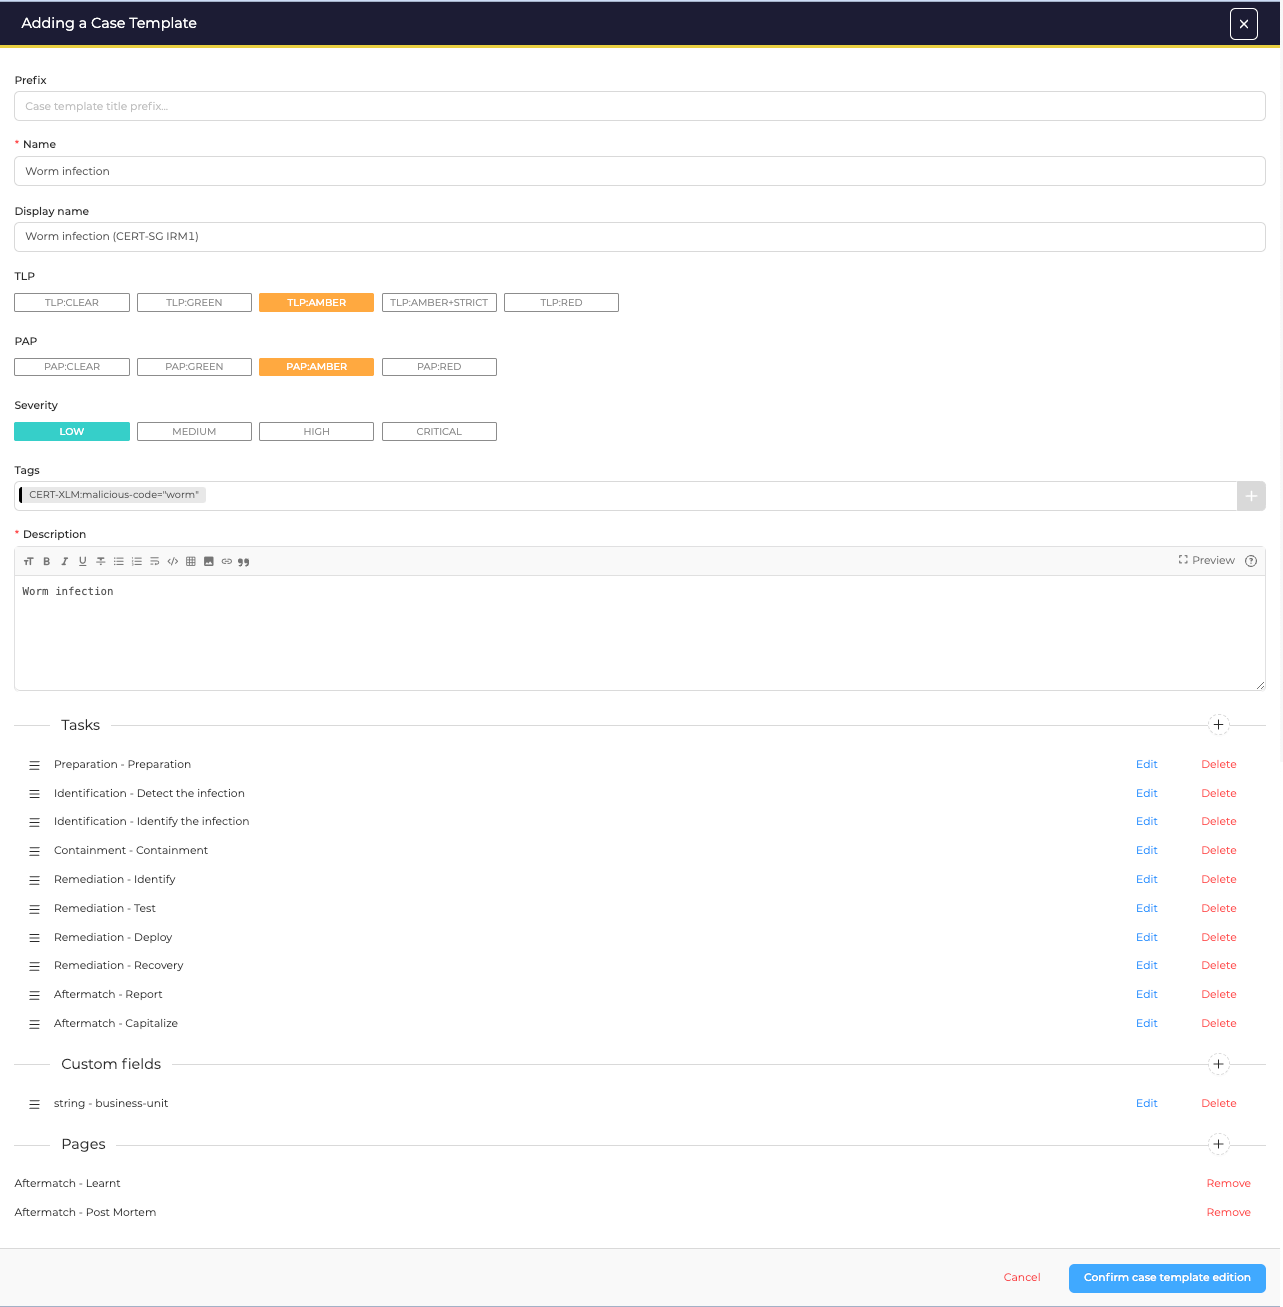
\includegraphics[width=0.8\textwidth]{img22.png}
    \caption{New Case template}
    \label{fig:new}
\end{figure}

\end{itemize}


\subsection*{Configuration parameters:}
When creating a Case template, the following parameters can be configured:

\begin{itemize}
  \item \textbf{Prefix}:A string that will be prepended to the title of a Case when it is created with this template.
  \item \textbf{Name}: The identifier of the Case template, utilized for recognition through the API.
  \item \textbf{Display Name}: The name of the Case template as presented in the UI.
  \item \textbf{TLP}: The default TLP (Traffic Light Protocol) of the Case when it is created with this template.
  \item \textbf{PAP}: The default PAP (Perceived Attribution Program) associated with the Case when created using this template.
  \item \textbf{Severity}:The default severity level assigned to the Case when created with this template.
  \item \textbf{Tags}: A list of tags that will be added to the Cases created with this template.
  \item \textbf{Description}: The default description assigned to Cases when they are created using this template if no modifications are made.
  \item \textbf{Tasks}: Tasks can be included in the templates, and they will be automatically integrated into the Case when it is created with this template.
  \item \textbf{Custom Fields}: Custom fields can be added to the template, with the option to set default values for these fields.
  \item \textbf{Pages}: Page templates can be added to the template, and they will be automatically included in the Case when it is created using this template.
\end{itemize}

\section*{Import and Export}

\subsection*{Exporting a Case Template}

Exporting a Case template involves the following steps:

\begin{enumerate}
  \item Click on the option icon, typically represented as three dots or a gear icon.
  \item Select ”Export case template” from the menu
\end{enumerate}

The Case template will be exported and saved as a JSON file. //

It is shown in Figure \ref{fig:export}.
\begin{figure}[h!]
    \centering
    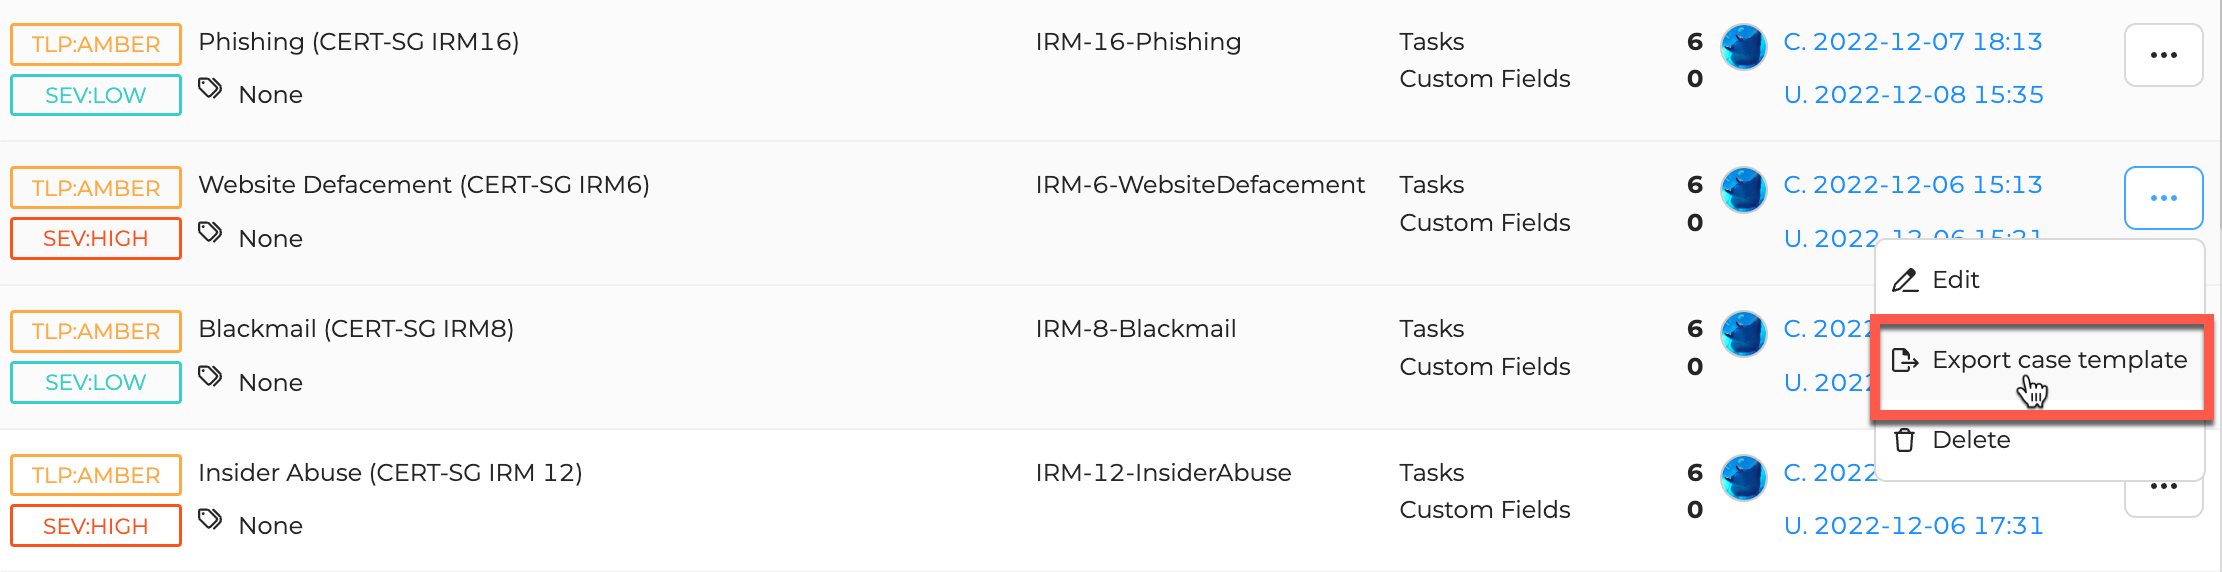
\includegraphics[width=0.8\textwidth]{img23.png}
    \caption{Export Case template}
    \label{fig:export}
\end{figure}

\subsection*{Importing a Case Template}

Importing a Case template involves the following steps:

\begin{enumerate}
  \item Click on the \textbf{Add a Case Template} button.
  \item Choose the JSON file that holds the Case template.
  \item Click "Confirm" to initiate the import of the Case template.
\end{enumerate}

It is shown in Figure \ref{fig:import}.
\begin{figure}[h!]
    \centering
    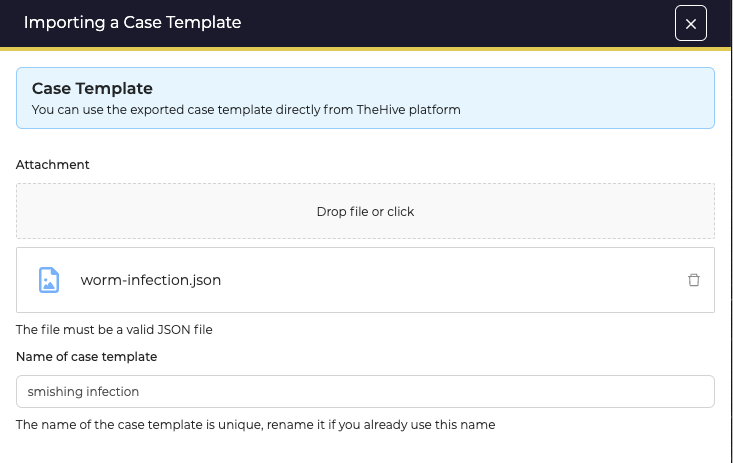
\includegraphics[width=0.8\textwidth]{img24.png}
    \caption{Import Case template}
    \label{fig:import}
\end{figure}

\subsection{Alerts}

Alerts serve as timely notifications that convey essential information regarding ongoing security issues, vulnerabilities, and potential exploits. They play a crucial role in keeping individuals and organizations informed about the current state of their digital security, enabling proactive responses to mitigate risks and address emerging threats promptly.

\subsubsection{View Alert Details}

To view the details of a specific alert, steps are the following:

\begin{enumerate}
  \item Navigate to the left menu and click on the "Alerts" button.
  \item Select the specific alert you wish to examine.
\end{enumerate}

Upon clicking on the alert, the Alerts page will show various tabs with additional details. These tabs include, the General tab, Observables, TTPs, Similar Cases, Similar Alerts, and the Responders tab. These tabs can be explored to gain a fine understanding of the alert and its associated information.

It is shown in Figure \ref{fig:alert}.

\begin{figure}[H]
    \centering
    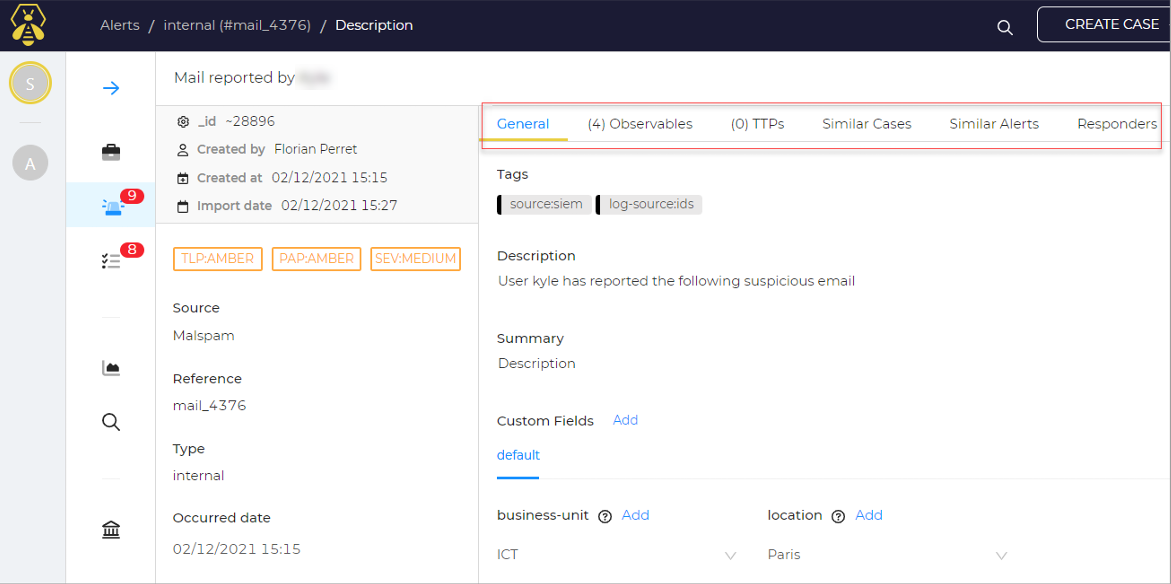
\includegraphics[width=0.8\textwidth]{img25.png}
    \caption{Alerts}
    \label{fig:alert}
\end{figure}

\subsubsection{Create a Case from an Alert}

The main page shows different alerts - some are new, and some are imported. You can only create a new case from the selection for the new alerts, making it easier to manage and respond to recently identified security issues.

It is shown in Figure \ref{fig:case}.
\begin{figure}[H]
    \centering
    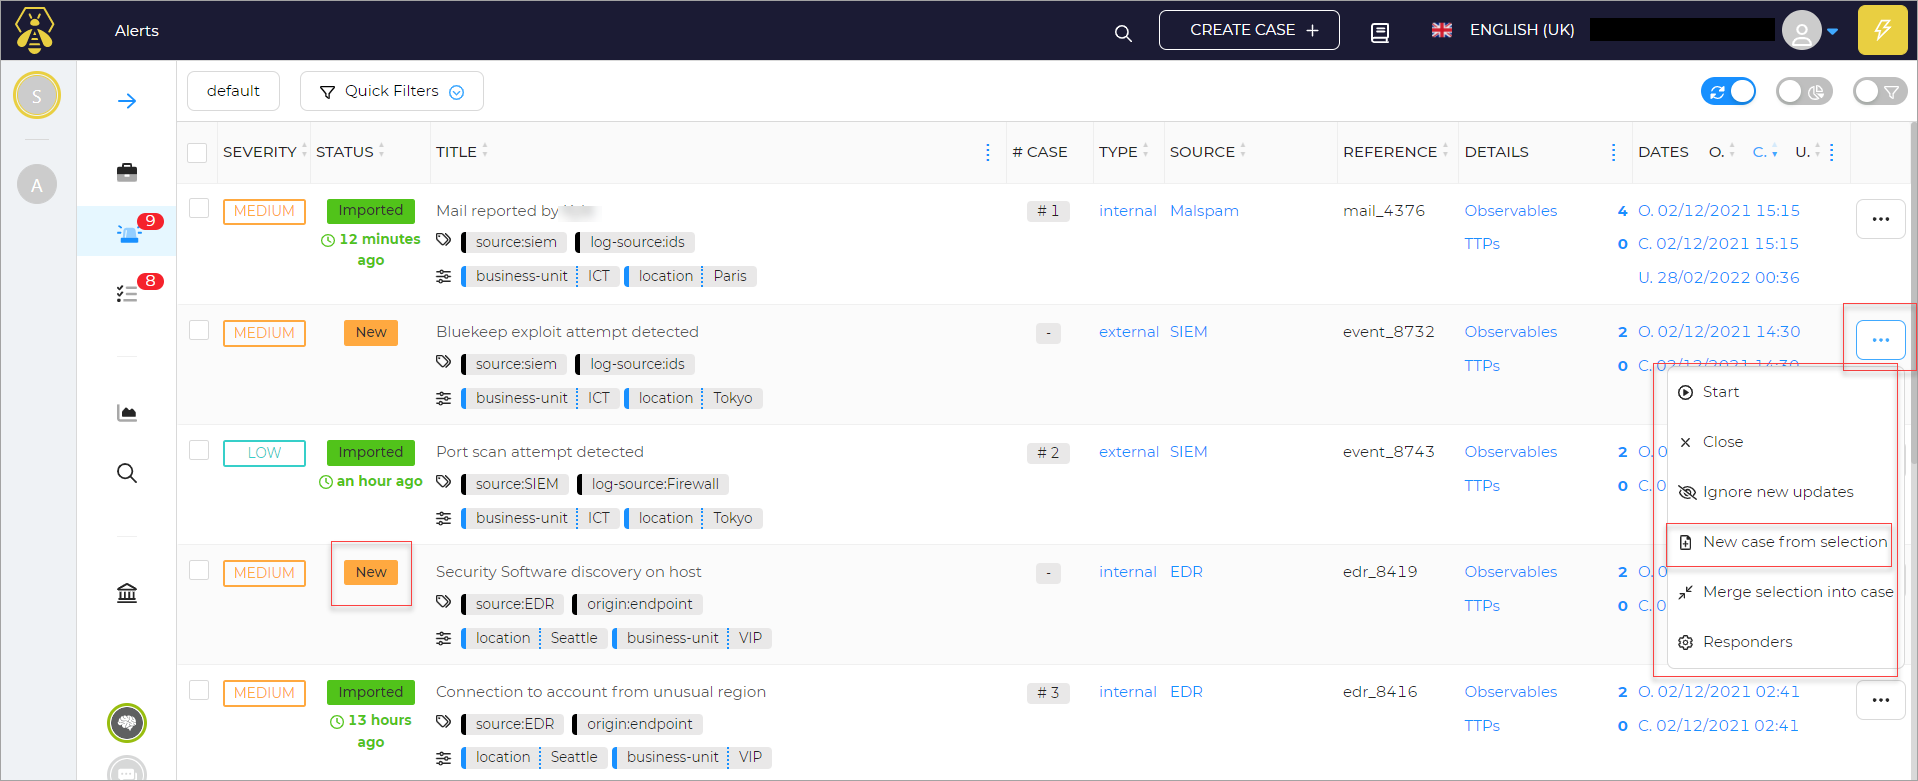
\includegraphics[width=0.8\textwidth]{img26.png}
    \caption{Create Case from Alert}
    \label{fig:case}
\end{figure}

To add a new case from a selection, follow these steps:

\begin{itemize}
  \item Navigate to the alert details page.
  \item Choose the alert for which you want to create a new case.
  \item Click on the "New Case from Selection" option.
  \item A new window will open, enabling you to easily create a new case based on your chosen alert.
\end{itemize}


When an empty case or a case template is chosen, a new case will be generated, incorporating the observables and Tactics, Techniques, and Procedures (TTPs) from the selected alert. This streamlines the process of case creation by automatically including relevant information from the alert into the new case.\\



\subsection{Seamless Collaboration with MISP}
TheHive is closely integrated with MISP (Malware Information Sharing Platform), significantly augmenting its capabilities in effectively managing and responding to security incidents. This tight integration ensures seamless collaboration and information sharing between the two platforms, enhancing overall incident handling and response capabilities.

\subsection{Stronger Analysis with Cortex Integration}
TheHive provides strong observable analysis by working closely with Cortex, another potent tool from TheHive Project. Cortex enables security experts to delve into detailed analysis of different observables, making incident response more effective through an easy-to-use web interface.\\

Highlights of observable analysis with Cortex include:


\begin{itemize}
  \item \textbf{Comprehensive Analysis Tools}:
  Cortex offers a diverse array of analyzers and responders, enabling thorough investigations on different observable types, including:
    \begin{itemize}
        \item IP addresses
        \item Email addresses
        \item URLs
        \item Domain names
        \item Files (e.g., attachments)
        \item Hashes (e.g., MD5, SHA-256)
        \item Registry keys (e.g., Windows Registry entries)
        \item And more...
    \end{itemize}
    These tools can reveal crucial information about potential threats associated with these observables.

  \item \textbf{Integration with TheHive}:
  we can initiate observable analysis directly from our incident cases, improving efficiency and reducing response times.
  
  \item \textbf{Automation}:
  Automate the analysis process by crafting analysis templates that define which analyzers to run for specific observable types. This automation simplifies your incident response workflow, making it more efficient.

  \item \textbf{Customization}: 
  We can customize Cortex by adding our own analyzers or responders to tailor the analysis capabilities to your organization's specific needs.
  
  \item \textbf{Scalability}: 
 Cortex is crafted to manage a large volume of observables, making it well-suited for organizations with extensive security operations.
  

\end{itemize}

\subsubsection{Analyzers and Responders}
When you go to the case details page, you can view all the cases associated with the organization.
It is shown in \ref{fig:cases}.
\begin{figure}[H]
    \centering
    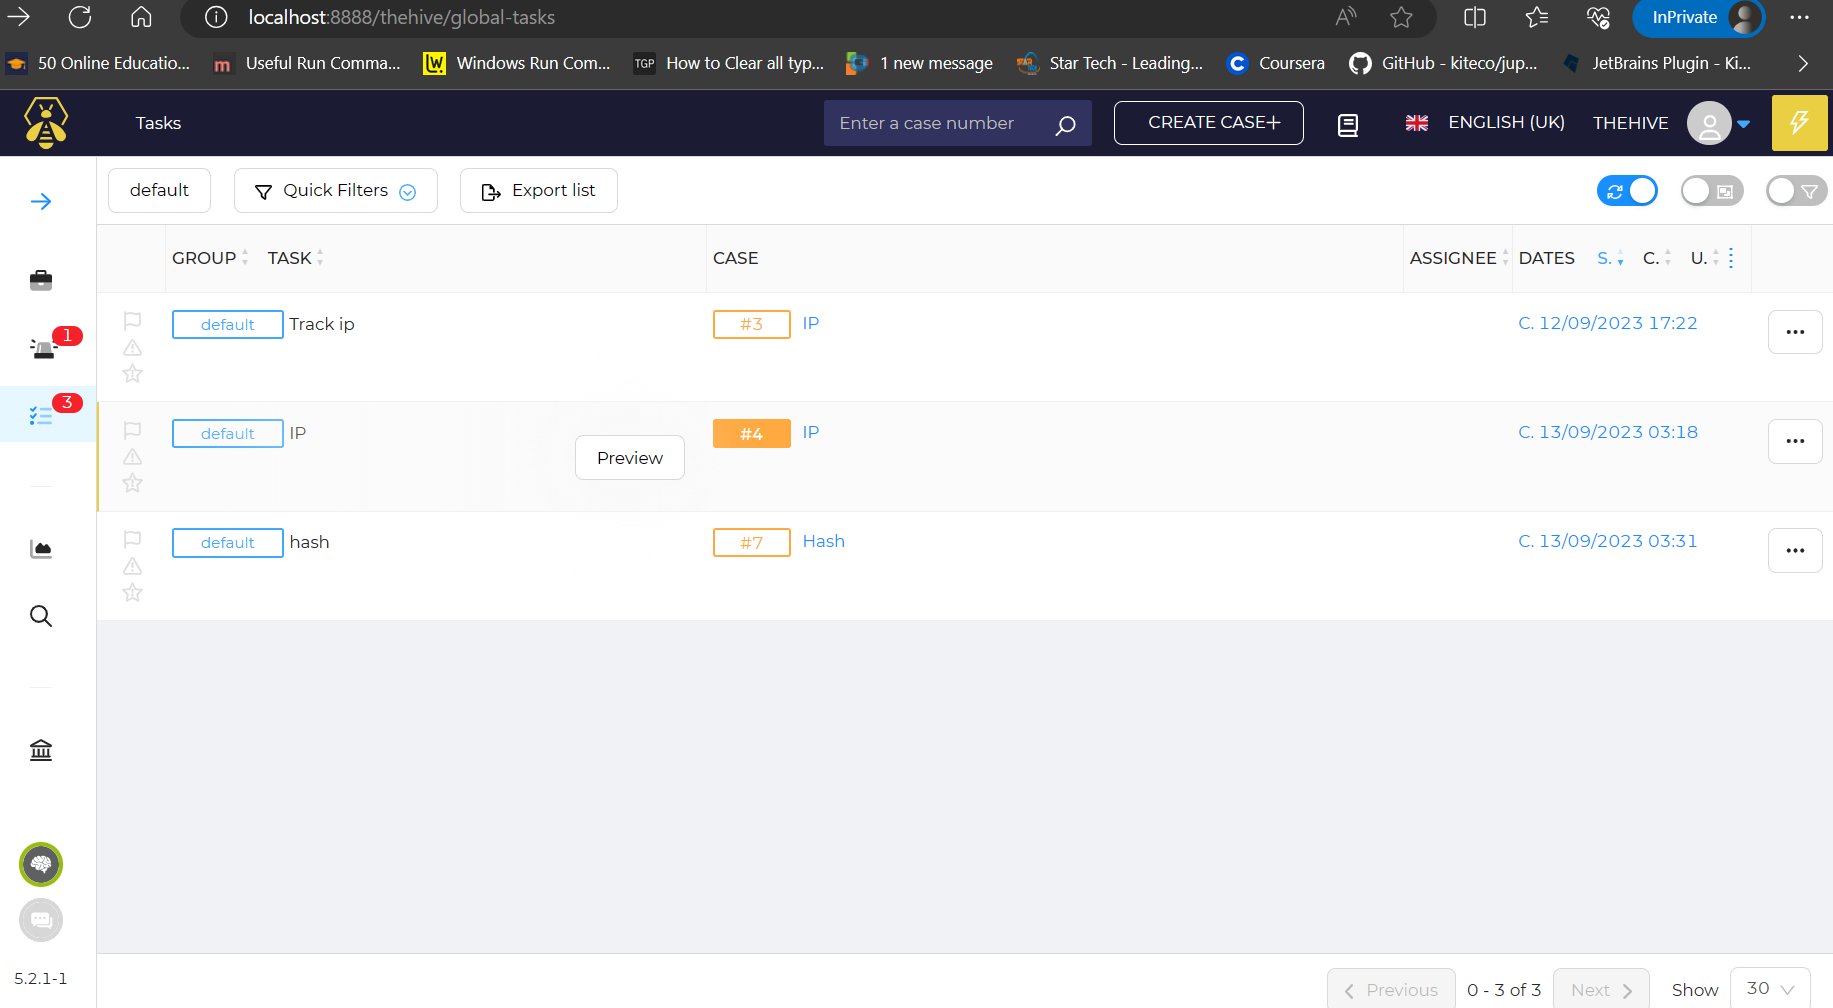
\includegraphics[width=0.8\textwidth]{img27.png}
    \caption{Cases}
    \label{fig:cases}
\end{figure}

 Click on the case you want to analyze. And then click on the \textbf{observables} tab of your task. It is shown in \ref{fig:observables}.

\begin{figure}[H]
    \centering
    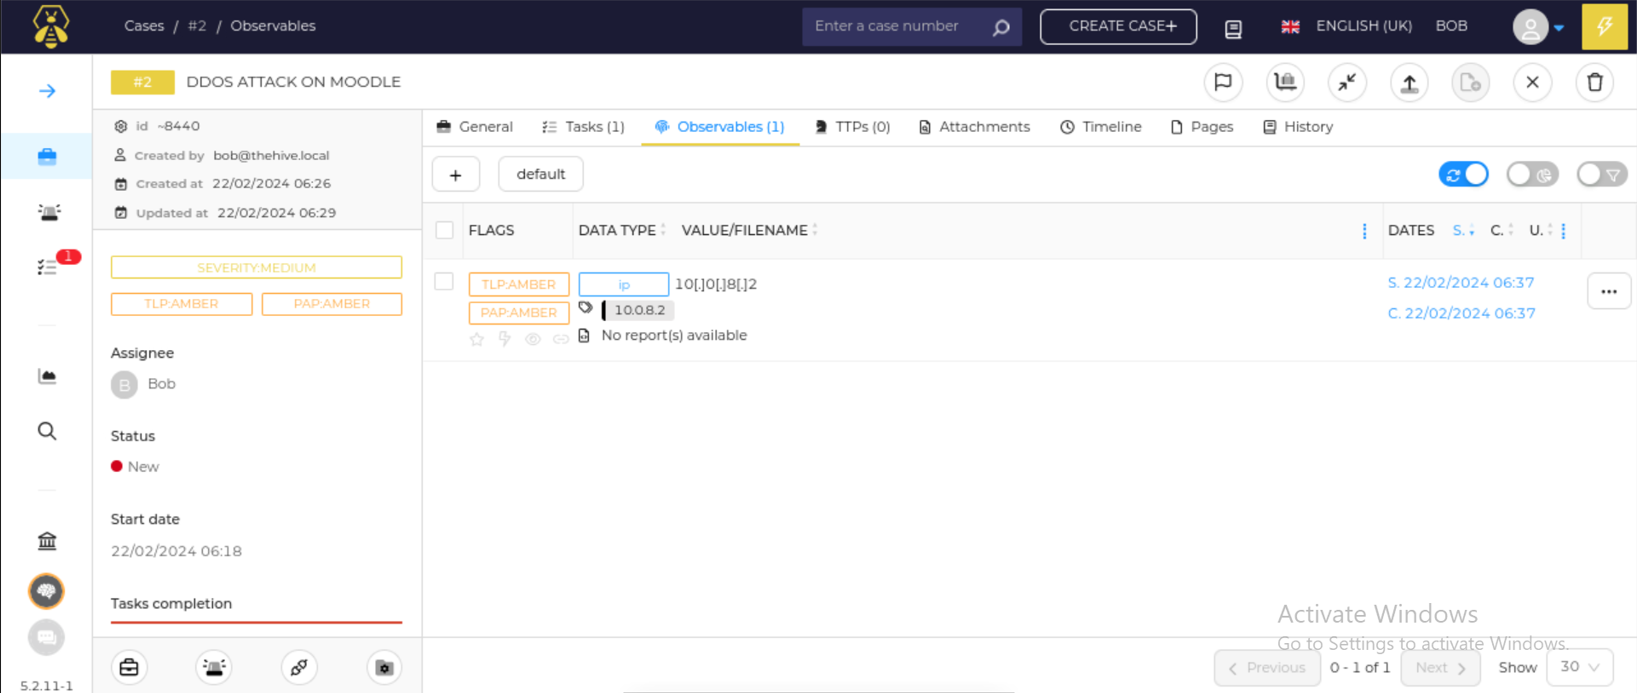
\includegraphics[width=0.8\textwidth]{img28.png}
    \caption{Observables}
    \label{fig:observables}
\end{figure}
 Currently, you can access all the observables related to the case and initiate the creation of new observables. To create an observable, you'll need to provide some essential basic information.
\begin{itemize}
    \item \textbf{Type}: Type of the observable.
    \item \textbf{Value}: Value of the observable.
    \item \textbf{Tags}: Tags of the observable, that will help us to search for the observable.
    \item \textbf{Description}
     \item \textbf{TLP}: TLP of the observable.
        \begin{itemize}
            \item \textbf{White} 
            \item \textbf{Green} 
            \item \textbf{Amber} 
            \item \textbf{Red} 
        \end{itemize}
    \item \textbf{PAP}: PAP of the observable.
        \begin{itemize}
            \item \textbf{White} 
            \item \textbf{Green} 
            \item \textbf{Amber} 
            \item \textbf{Red} 
        \end{itemize}
\end{itemize}

\subsubsection{Analyzers}
Cortex offers an extensive selection of analyzers for diverse analysis needs. We can get the whole list of analyzer and there task in Cortex. This is shown in \ref{fig:analyzersList}. Once the observable is created, you'll encounter the analyzers option. For instance, if you're working with an IP address observable, you can observe the available analyzers. \ref{fig:analyzers} displays the list of analyzers.\\

\begin{figure}[H]
    \centering
    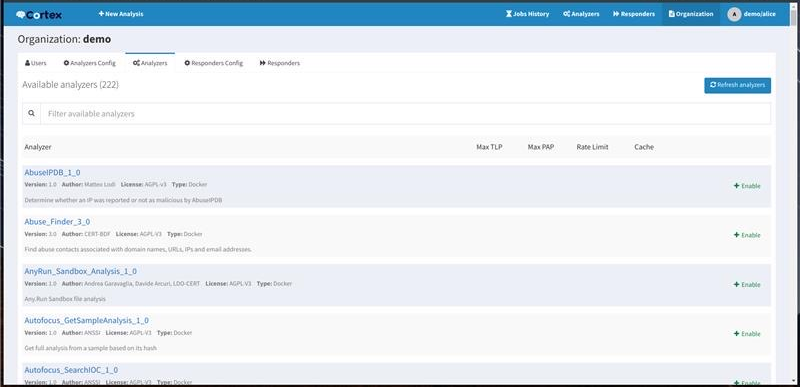
\includegraphics[width=0.8\textwidth]{img33.png}
    \caption{Analyzers}
    \label{fig:analyzersList}
\end{figure}

\begin{figure}[H]
    \centering
    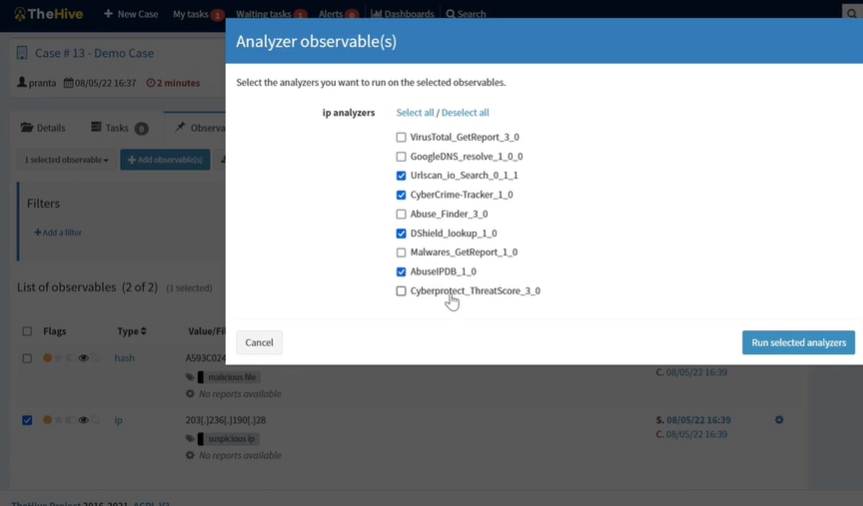
\includegraphics[width=0.8\textwidth]{img30.png}
    \caption{Analyzers}
    \label{fig:analyzers}
\end{figure}

Cortex provides a wide range of analyzers such as:
\begin{itemize}
    \item \textbf{Abuse Finder}
    \item \textbf{Google DNS Resolver}
    \item \textbf{URL Scan}
    \item \textbf{Cyber Protect Threat Score}
\end{itemize}

Another example is shown in \ref{fig:analyzers2} . Here we can see the available analyzers for hash observable.
\begin{figure}[H]
    \centering
    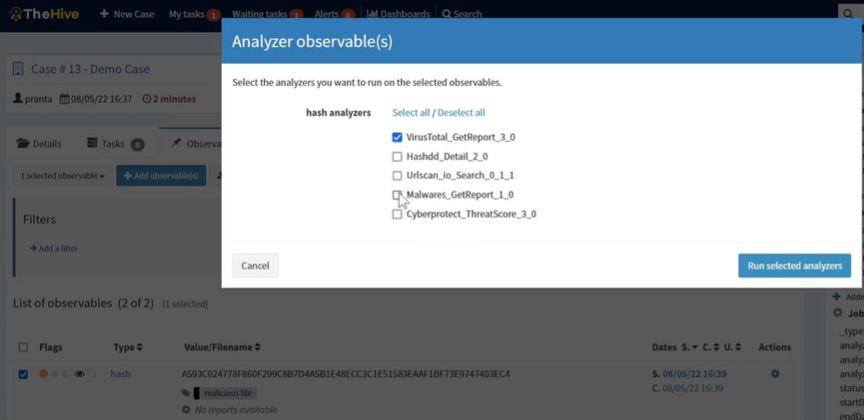
\includegraphics[width=0.8\textwidth]{img29.png}
    \caption{Analyzers}
    \label{fig:analyzers2}
\end{figure}

\ref{fig:analyzers2}.


\subsubsection{Analysis Report}
After running the analyzer, we can see the analysis report. Here danger levels are shown with results from different analyzers \textbf{Color Coded}.
For example, we can see the analysis report of the hash observable.
It is shown in \ref{fig:analysis-report}. Two blue colors indicate that, according to that particular analyzer, the hash is not considered malicious. Conversely, two red colors indicate that the hash is identified as malicious by that specific analyzer.
\begin{figure}[H]
    \centering
    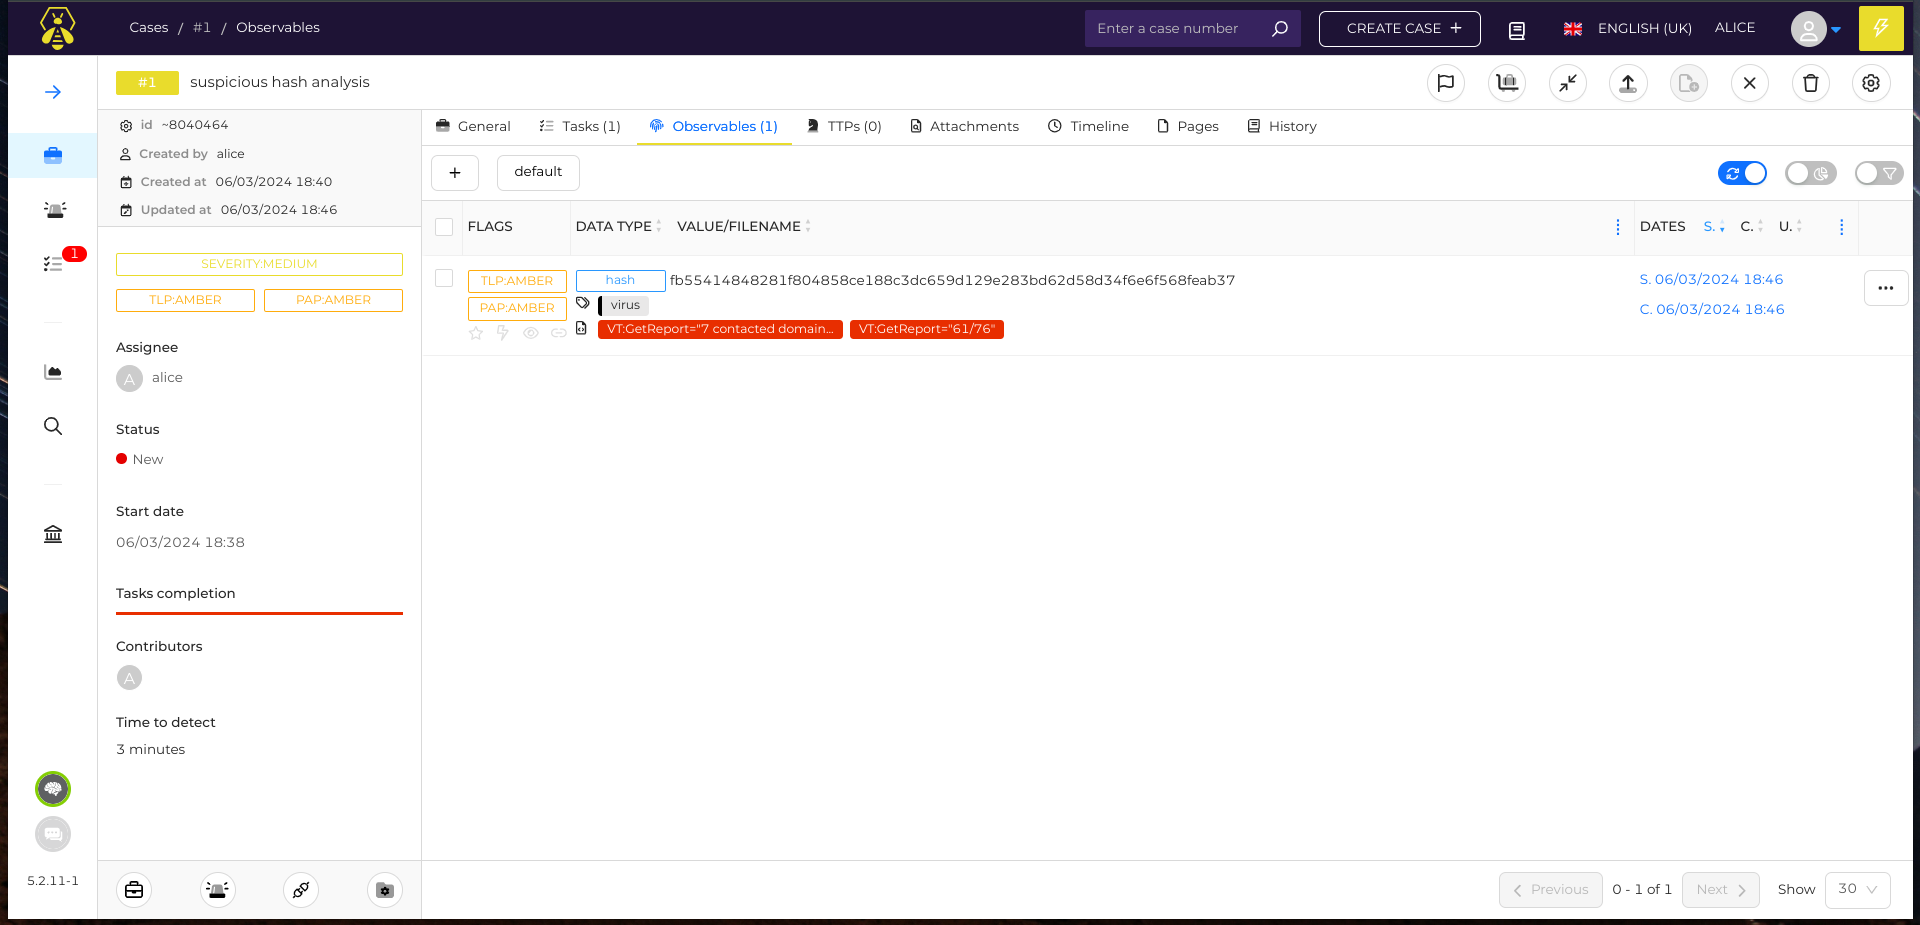
\includegraphics[width=0.8\textwidth]{img35.png}
    \caption{Analysis Report}
    \label{fig:analysis-report}
\end{figure}
We can see the report in details at \ref{fig:analysis-report2}

\begin{figure}[H]
    \centering
    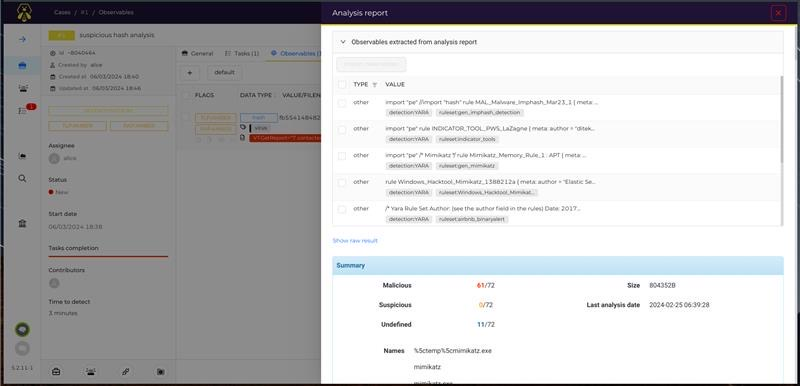
\includegraphics[width=0.8\textwidth]{img34.png}
    \caption{Analysis Report}
    \label{fig:analysis-report2}
\end{figure}

We can see the Job history from Cortex where all the analyzers result run on the observables are saved. See this in \ref{fig:job-history}
Here We can see the job details per observable and find report in JSON format. It is shown in \ref{fig:cortex-report}

\begin{figure}[H]
    \centering
    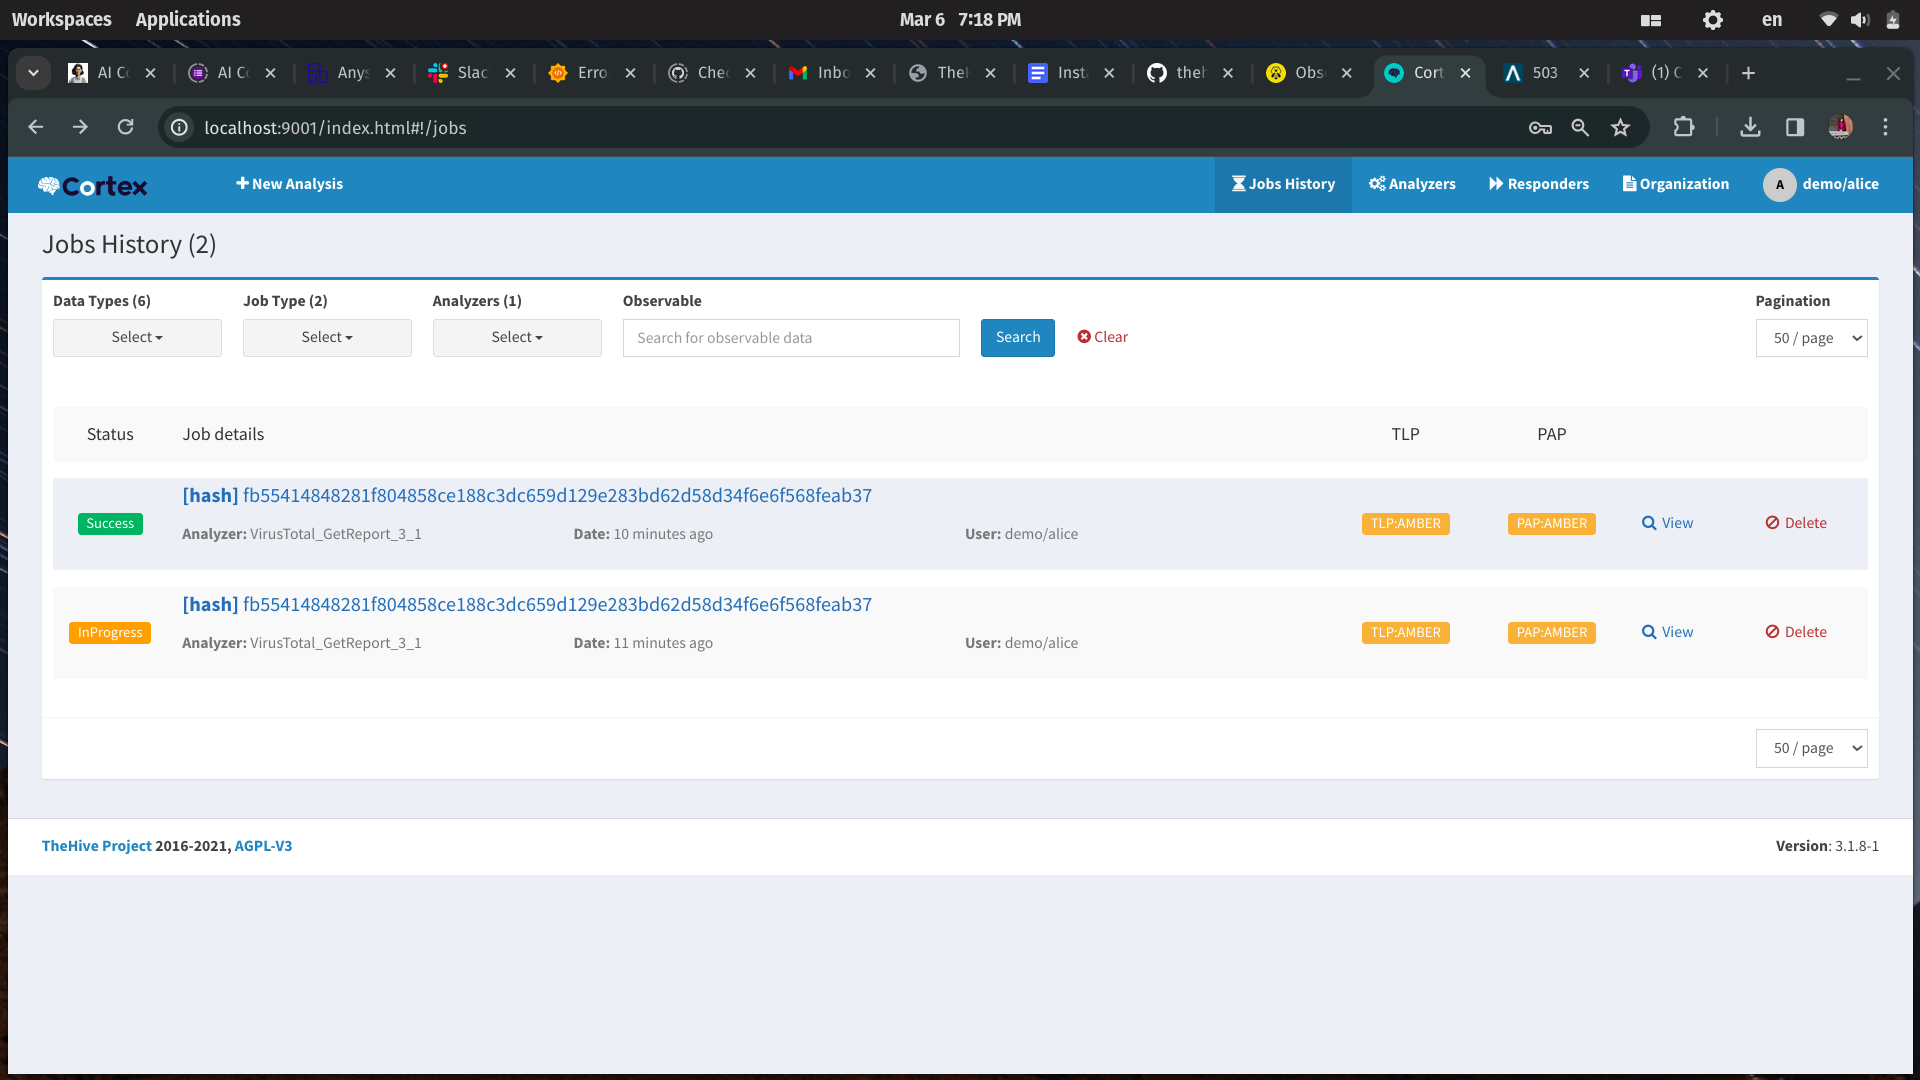
\includegraphics[width=0.8\textwidth]{img39.png}
    \caption{Job History}
    \label{fig:job-history}
\end{figure}

\begin{figure}[H]
    \centering
    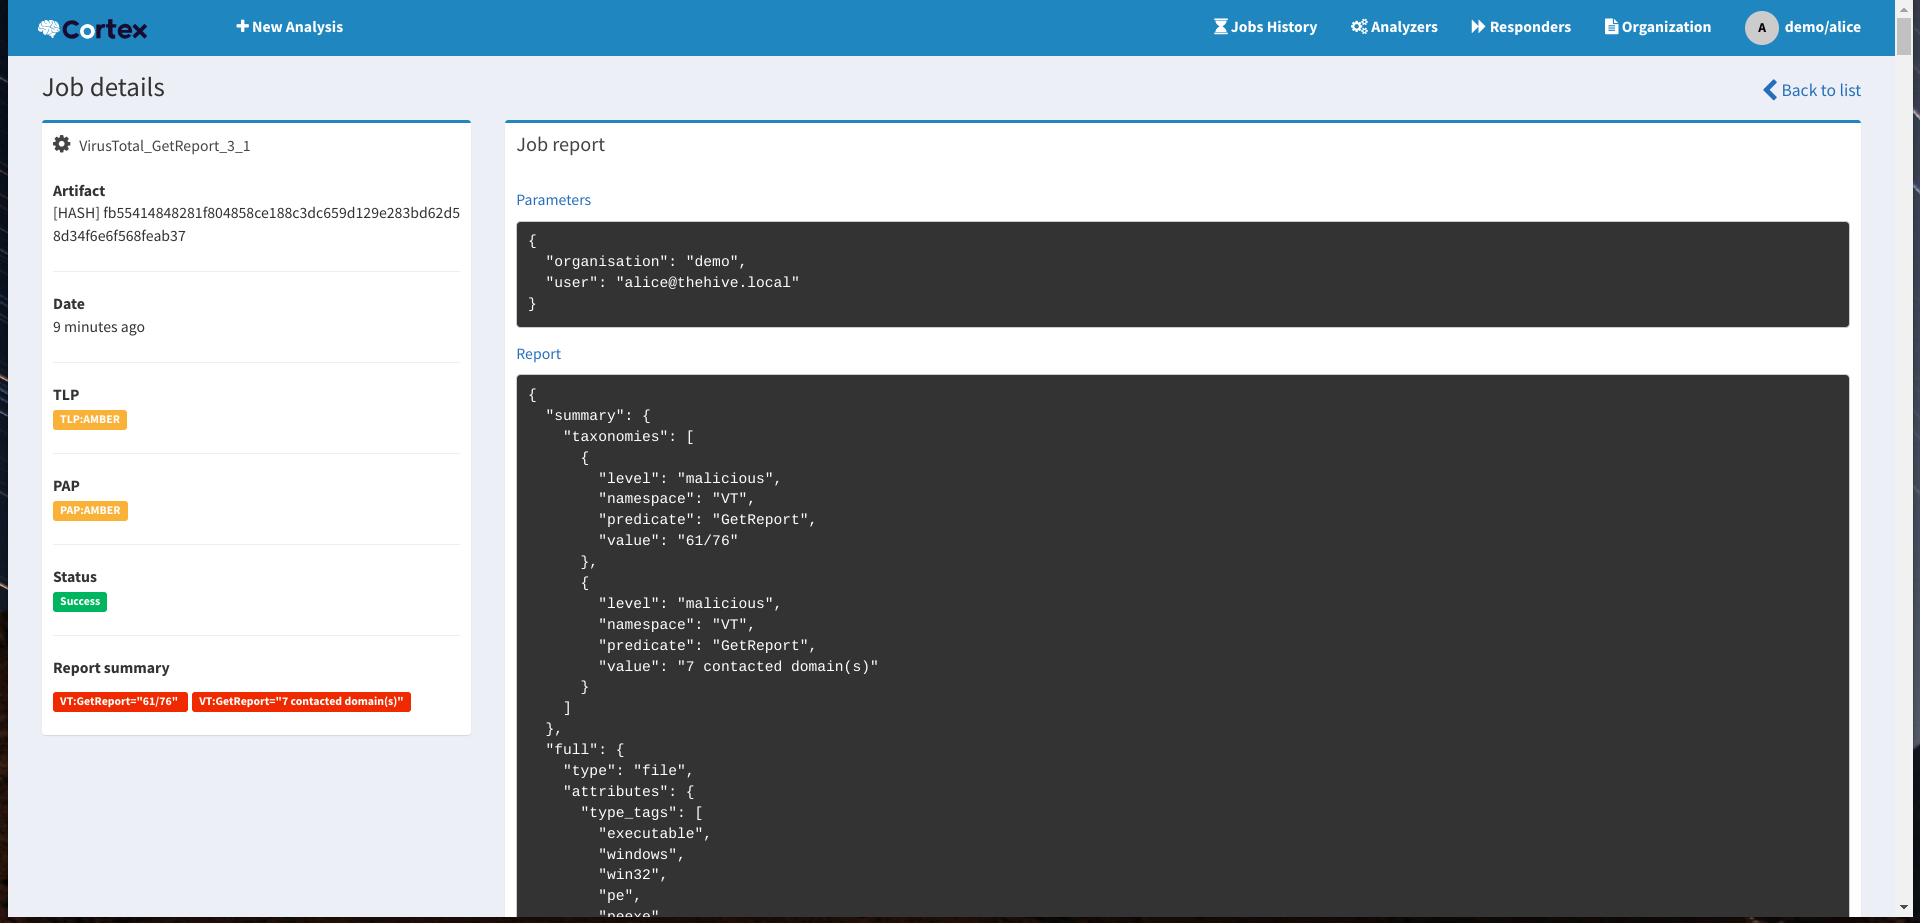
\includegraphics[width=0.8\textwidth]{img36.png}
    \caption{Analysis Report}
    \label{fig:cortex-report}
\end{figure}


\section{Use Cases}
Here we can discuss some specific use cases where TheHive excels.

\begin{itemize}
    \item \textbf{Incident management:} TheHive streamlines efficient security incident management by offering a centralized platform. It facilitates the creation of cases, assignment of tasks, and real-time tracking of investigation progress.
     \item \textbf{Automation:} Leverage The Hive's integration with Cortex for automating incident response processes. Cortex, a potent engine, allows the analysis of observables like IP addresses, email addresses, URLs, domain names, files, or hashes through a user-friendly web interface. Automation extends to large sets of observables from TheHive, Cortex REST API, alternative SIRP platforms, custom scripts, or MISP.
    \item \textbf{Collaboration:}  Enhance collaboration with other teams using TheHive. Share information on security incidents, create alerts, exchange observables, and communicate seamlessly with other teams in real-time.
    \item \textbf{Reporting:} TheHive provides comprehensive reports on incident response activities. Generate detailed reports on metrics such as the number of cases created, tasks assigned, and the overall progress of investigations.
\end{itemize}


\section{Conclusion}
The Hive stands out as a potent and adaptable Security Incident Response System (SIRS) suitable for organizations of all sizes. It undergoes continuous updates, introducing new features and enhancements. With a flexible architecture and a user-friendly interface, it equips security teams with the necessary tools for efficient orchestration of incident response processes. The platform's automation capabilities, seamless integration with external security tools, and comprehensive reporting and analytics empower security professionals to streamline their workflows. Overall, in the face of evolving threat landscapes, The Hive remains a valuable asset, enhancing organizational security posture, streamlining incident response, and promoting a proactive cybersecurity approach.

\end{document}
```

This is just a basic outline. You can add more sections or details as needed. Remember to replace "Your Name" with your actual name. Happy writing!